\documentclass[11pt]{article}

\usepackage[margin=0.82in]{geometry}
\usepackage{amsmath,amssymb}
\usepackage{booktabs}
\usepackage{graphicx}
\usepackage[table]{xcolor}
\usepackage{float}
\usepackage{enumitem}
\usepackage{microtype}
\usepackage[hidelinks]{hyperref}

\setlength{\parindent}{0pt}
\setlength{\parskip}{0.4em}
\setlength{\intextsep}{8pt plus 2pt minus 2pt}
\setlength{\abovecaptionskip}{5pt}
\setlength{\belowcaptionskip}{0pt}
\setlist[itemize]{topsep=2pt,itemsep=1.5pt,parsep=0pt,leftmargin=1.2em}
\setlist[enumerate]{topsep=2pt,itemsep=1.5pt,parsep=0pt,leftmargin=1.6em}

% Every comparison is written as a higher-is-better performance improvement,
% PE - Standard, so positive favors PE. Green is PE ahead and red is Standard ahead; the deeper tint plus
% bold type marks the cells whose 95% interval also excludes zero.
\newcommand{\pewin}[1]{\cellcolor{green!22}$\mathbf{#1}$}
\newcommand{\pesoft}[1]{\cellcolor{green!8}$#1$}
\newcommand{\stdwin}[1]{\cellcolor{red!18}$\mathbf{#1}$}
\newcommand{\stdsoft}[1]{\cellcolor{red!6}$#1$}
\newcommand{\setup}{\textbf{Setup.}\ }
\newcommand{\findings}{\textbf{Findings.}}

\title{Probabilistic Exploration for Efficient Bayesian Optimization}
\author{Jungwoo Hong}
\date{}

\begin{document}
\maketitle

\section{Research questions, conclusions, and protocol}

This report addresses three research questions. First, does PE help
beyond a single objective or acquisition function? Second, can the decay
exponent $\alpha$ be related to dimension or selected reliably from a small
pilot? Third, can a more evenly spaced exploration design improve on Uniform
sampling? Sections~\ref{sec:acq}--\ref{sec:dimalpha} address the first question,
Section~\ref{sec:choice} addresses the second, and
Sections~\ref{sec:external} and \ref{sec:hpo} test transfer to Lunar Lander
controller tuning and hyperparameter optimisation. Section~\ref{sec:packing}
addresses the third question.

\textbf{Main conclusions.} PE improves GP-UCB, LogEI, and MES-Gumbel on
multiple 30D objectives. With the theory-aligned GP-TS implementation, the
benefit repeats on Rosenbrock but not on Bent Cigar or Sparse Hartmann. Useful exponents are usually between
$1/2$ and $1$, yet neither dimension nor a small seed sweep identifies a
reliable winner. On Lunar Lander, Decay PE gives a clear and transferable gain
with LogEI. In 14D YAHPO tuning, Decay PE helps several UCB, LogEI, and MES
settings, mainly by reducing high-loss failures on one dataset. In 28D, decay
$\alpha=1/2$ improves LogEI and GP-TS on \texttt{sylvine}, but most other cells
remain tied or inconclusive. The current evidence therefore supports PE as a
useful option, but does not yet support a universal rule for choosing $\alpha$.
Finite-grid Greedy Packing is strongly problem-dependent. It helps Rastrigin,
especially in 10D and 30D, and preserves PE gains for several 30D Sparse
Hartmann acquisitions. It also gives selective gains on 28D YAHPO, while both
Uniform and Greedy PE improve over Standard on Lunar. However, the same
schedule transfers poorly to Ackley and Rosenbrock, and a fourfold larger grid
does not remove this dependence. Greedy is therefore less reliable than
Uniform PE as a default.

\textbf{Protocol.} GP signal variance fixed to $1$ and not learned, so
$k(x,x)\le 1$; lengthscales learned; GP inputs mapped to $[0,1]^d$; scrambled
Sobol initial design. Within each benchmark, acquisition, and seed all compared
policies share the same initial observations and observation-noise stream, so
every comparison is paired. The decay family is
$p_t=\log(t+1)/(t+1)^{\alpha}$ with $t$ the one-based BO step after the initial
design, so a smaller $\alpha$ keeps PE active for more steps.
For GP-TS, the previous fixed-$\beta$ result is replaced throughout by
$\beta_t=\log(t+1)$ and a fresh scrambled-Sobol discretization of size
$\operatorname{clip}(\lceil64\sqrt{t}\rceil,128,512)$ at BO step $t$.

\textbf{Reading the numbers.} Define a higher-is-better performance score as
$s=-\text{regret}$ on synthetic benchmarks and $s=\text{return}$ on Lunar. All
comparisons then use one convention:
\[
  \text{improvement over Standard} \;=\; s(\text{PE})-s(\text{Standard}).
\]
Equivalently, this is Standard regret minus PE regret on synthetic objectives,
and PE return minus Standard return on Lunar. Thus positive always favors PE.
Uncertainty is a paired bootstrap 95\% confidence
interval on that difference. Green favors PE and red favors Standard. A deep,
bold cell has an interval that excludes zero; a pale cell does not. Figures use
filled markers or outlined heatmap cells for the same distinction. Intervals
are not corrected for the simultaneous comparisons in a row, and any cell
labelled ``best'' was selected and evaluated on the same seeds unless a
held-out split is stated explicitly.

\begin{table}[H]
\centering
\scriptsize
\begin{tabular}{@{}p{0.43\textwidth}llll@{}}
\toprule
Experiment & $\sigma_f^2$ & $n_{\mathrm{initial}}$ & BO seeds & Eval. steps \\
\midrule
Rastrigin dimension--$\alpha$ sweep, Uniform and MVR & $1$ & $2d$ & 5 & $400+2d$ \\
Rastrigin dimension--$\alpha$ sweep, Uniform & $1$ & 2 & 5 & 402 \\
Rastrigin held-out confirmation of the selected $\alpha$ & $1$ & 2 & 15 & 402 \\
Rosenbrock and Ackley dimension--$\alpha$ panels & $1$ & 2 & 5 & 402 \\
30D acquisition sweep, three objectives & $1$ & 60 & 5 & 500 \\
30D acquisition sweep, two objectives & $1$ & 2 & 5 & 500 \\
30D acquisition held-out confirmation & $1$ & 2 & 10 & 500 \\
30D acquisition held-out, exponents $1/2$ and $4/3$ & $1$ & 2 & 10 & 500 \\
Rastrigin dimension--$\alpha$ sweep at 35 seeds & $1$ & 2 & 35 & 402 \\
Lunar Lander 12D, four completed acquisitions & $1$ & 24 & 30 & 400 \\
Lunar held-out controller evaluation & -- & -- & 30 & 200 episodes/controller \\
YAHPO XGBoost 14D, three tasks and four acquisitions & $1$ & 10 & 30 & 120 \\
YAHPO 28D, two tasks and four acquisitions & $1$ & 10 & 30 & 200 \\
Greedy Packing, 30D acquisition comparison & $1$ & 2 & 10 & 500 \\
Greedy Packing, Rastrigin 2D--30D & $1$ & 2 & 15 & 402 \\
Greedy Packing, selected-setting validation & $1$ & 2 & 10 & 402 \\
Greedy Packing, Ackley and Rosenbrock transfer & $1$ & 2 & 5 & 402 \\
Greedy Packing, YAHPO 14D and 28D & $1$ & 10 & 30 & 120 / 200 \\
Greedy Packing, Lunar Lander 12D & $1$ & 24 & 30 & 400 \\
Fourfold-grid synthetic confirmation & $1$ & 2 & 15 & 200 \\
Fourfold-grid YAHPO confirmation & $1$ & 10 & 15 & 120 / 200 \\
Larger-grid Lunar confirmation & $1$ & 24 & 15 & 400 \\
\bottomrule
\end{tabular}

\caption{Stages reported here; all passed completeness and protocol audits.
Evaluation steps include the initial design. The Lunar held-out row is a
separate evaluation of saved controllers, not another BO run.}
\label{tab:scope}
\end{table}

\section{Does PE help across acquisition functions in 30D?}
\label{sec:acq}

\setup Three 30D objectives (Sparse Hartmann-6, Rosenbrock, Shifted Bent Cigar)
$\times$ four acquisitions (GP-UCB, GP-TS, LogEI, MES-Gumbel) $\times$ six
policies: Standard, Decay Uniform at $\alpha=1/2$, $2/3$, $1$ and $4/3$, and
Fixed $p=0.2$ as a schedule-free control. LogEI represents the EI family and
MES-Gumbel the entropy family. We use 500 evaluation steps and ten paired seeds
throughout. Averaged over the completed runs, $\alpha=1/2$ uses 191 random
queries, $\alpha=2/3$ uses 83, $\alpha=1$ uses 21, and $\alpha=4/3$ uses 6,
against 97 for Fixed $p=0.2$.

\begin{figure}[H]
  \centering
  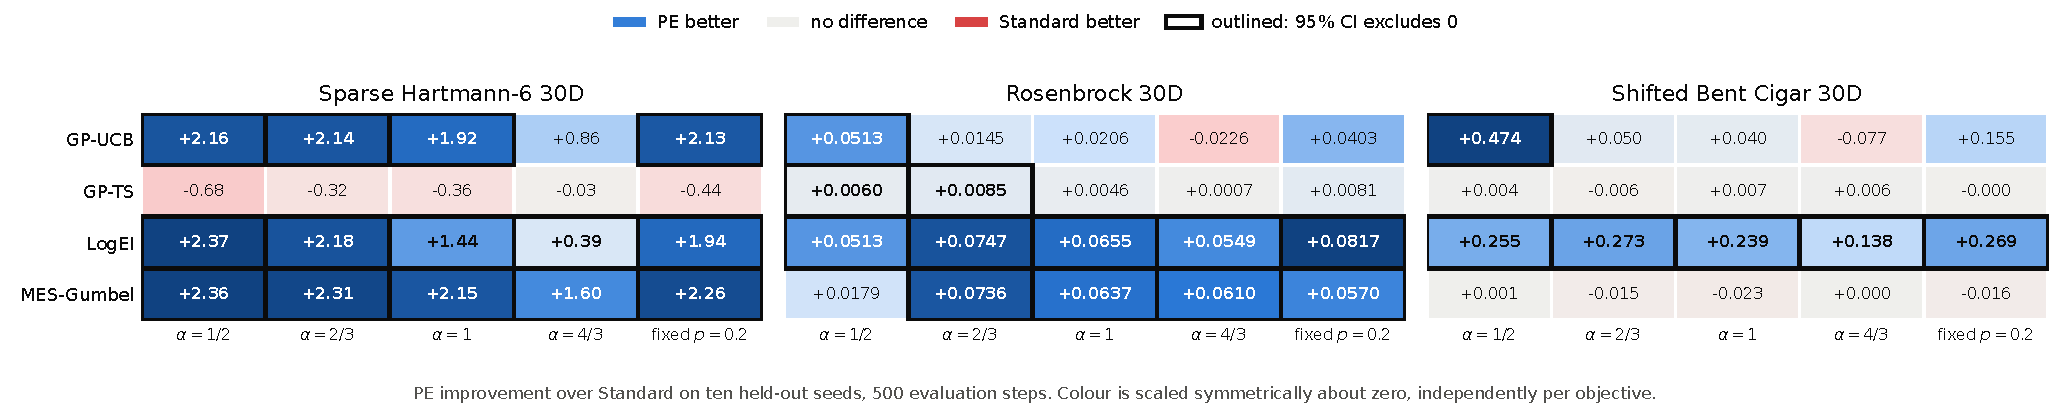
\includegraphics[width=\textwidth]{figures/fig_acquisition_30d_endpoint_heatmap.pdf}
  \caption{Endpoint improvement over Standard for every objective, acquisition
  and PE arm.}
  \label{fig:acqall}
\end{figure}

\begin{table}[H]
\centering
\small
\begin{tabular}{@{}llrlrlr@{}}
\toprule
 & & \multicolumn{2}{c}{$\alpha=2/3$ (reference)} & \multicolumn{3}{c}{$\alpha=1/2$ (slowest decay)} \\
\cmidrule(lr){3-4}\cmidrule(l){5-7}
Objective & Acquisition & Improv. & Wins & Improv. & 95\% CI & Wins \\
\midrule
Sparse Hartmann-30 & GP-UCB & \pewin{2.140} & 9/10 & \pewin{2.162} & $[1.296, 2.941]$ & 10/10 \\
 & GP-TS & \stdsoft{-0.315} & 4/10 & \stdsoft{-0.679} & $[-1.661, 0.456]$ & 3/10 \\
 & LogEI & \pewin{2.180} & 9/10 & \pewin{2.373} & $[1.596, 2.939]$ & 10/10 \\
 & MES-Gumbel & \pewin{2.307} & 9/10 & \pewin{2.356} & $[1.535, 2.956]$ & 10/10 \\
\addlinespace
Rosenbrock-30 & GP-UCB & \pesoft{0.0145} & 6/10 & \pewin{0.0513} & $[0.0145, 0.0994]$ & 9/10 \\
 & GP-TS & \pewin{0.0085} & 7/10 & \pewin{0.0060} & $[0.0001, 0.0120]$ & 7/10 \\
 & LogEI & \pewin{0.0747} & 10/10 & \pewin{0.0513} & $[0.0138, 0.0890]$ & 8/10 \\
 & MES-Gumbel & \pewin{0.0736} & 9/10 & \pesoft{0.0179} & $[-0.0383, 0.0757]$ & 5/10 \\
\addlinespace
Bent Cigar-30 & GP-UCB & \pesoft{0.050} & 4/10 & \pewin{0.474} & $[0.202, 0.806]$ & 9/10 \\
 & GP-TS & \stdsoft{-0.0057} & 5/10 & \pesoft{0.0041} & $[-0.0041, 0.0133]$ & 6/10 \\
 & LogEI & \pewin{0.273} & 10/10 & \pewin{0.255} & $[0.163, 0.339]$ & 9/10 \\
 & MES-Gumbel & \stdsoft{-0.0152} & 3/10 & \pesoft{0.0010} & $[-0.0191, 0.0216]$ & 5/10 \\
\bottomrule
\end{tabular}

\caption{The slowest exponent in the sweep against $\alpha=2/3$.}
\label{tab:acqall}
\end{table}

\findings
\begin{itemize}
  \item Three of the four acquisitions have positive mean improvements on all
        three objectives once the decay is slow enough. LogEI does so at
        $\alpha=2/3$; GP-UCB and MES-Gumbel need $\alpha=1/2$ on at least one
        objective. Not every individual interval excludes zero.
  \item \textbf{For GP-UCB, the conclusion changes with the exponent.} At
        $\alpha=2/3$ GP-UCB gains only on Sparse Hartmann. At $\alpha=1/2$ it
        gains on all three: Rosenbrock moves from $0.0145$ with a straddling
        interval to $0.0513$ $[0.0145, 0.0994]$ at 9/10 seeds, and Bent Cigar
        from $0.050$ at 4/10 to $0.474$ $[0.202, 0.806]$ at 9/10, a tenfold
        difference in the same cell.
  \item The improvement tends to decline as $\alpha$ increases. Among the four decay arms,
        $\alpha=1/2$ is strongest in seven of the twelve
        objective--acquisition cells and $\alpha=4/3$ weakest in eight.
  \item Under the replacement GP-TS, Rosenbrock improves at $\alpha=1/2$
        ($0.0060$) and $\alpha=2/3$ ($0.0085$), with both paired intervals
        above zero on the ten held-out seeds. Bent Cigar and Sparse Hartmann
        have no clear GP-TS gain.
  \item MES-Gumbel on Bent Cigar is the one block where no arm has a clear
        gain; every interval contains zero.
  \item Fixed $p=0.2$ tracks $\alpha=2/3$, whose exploration budget it nearly
        matches: the two share a sign in eleven of twelve cells and their
        intervals overlap in all twelve. Because their query counts are close
        but not exactly matched, this comparison alone cannot separate the
        effect of timing from the total amount of exploration.
\end{itemize}

\begin{figure}[H]
  \centering
  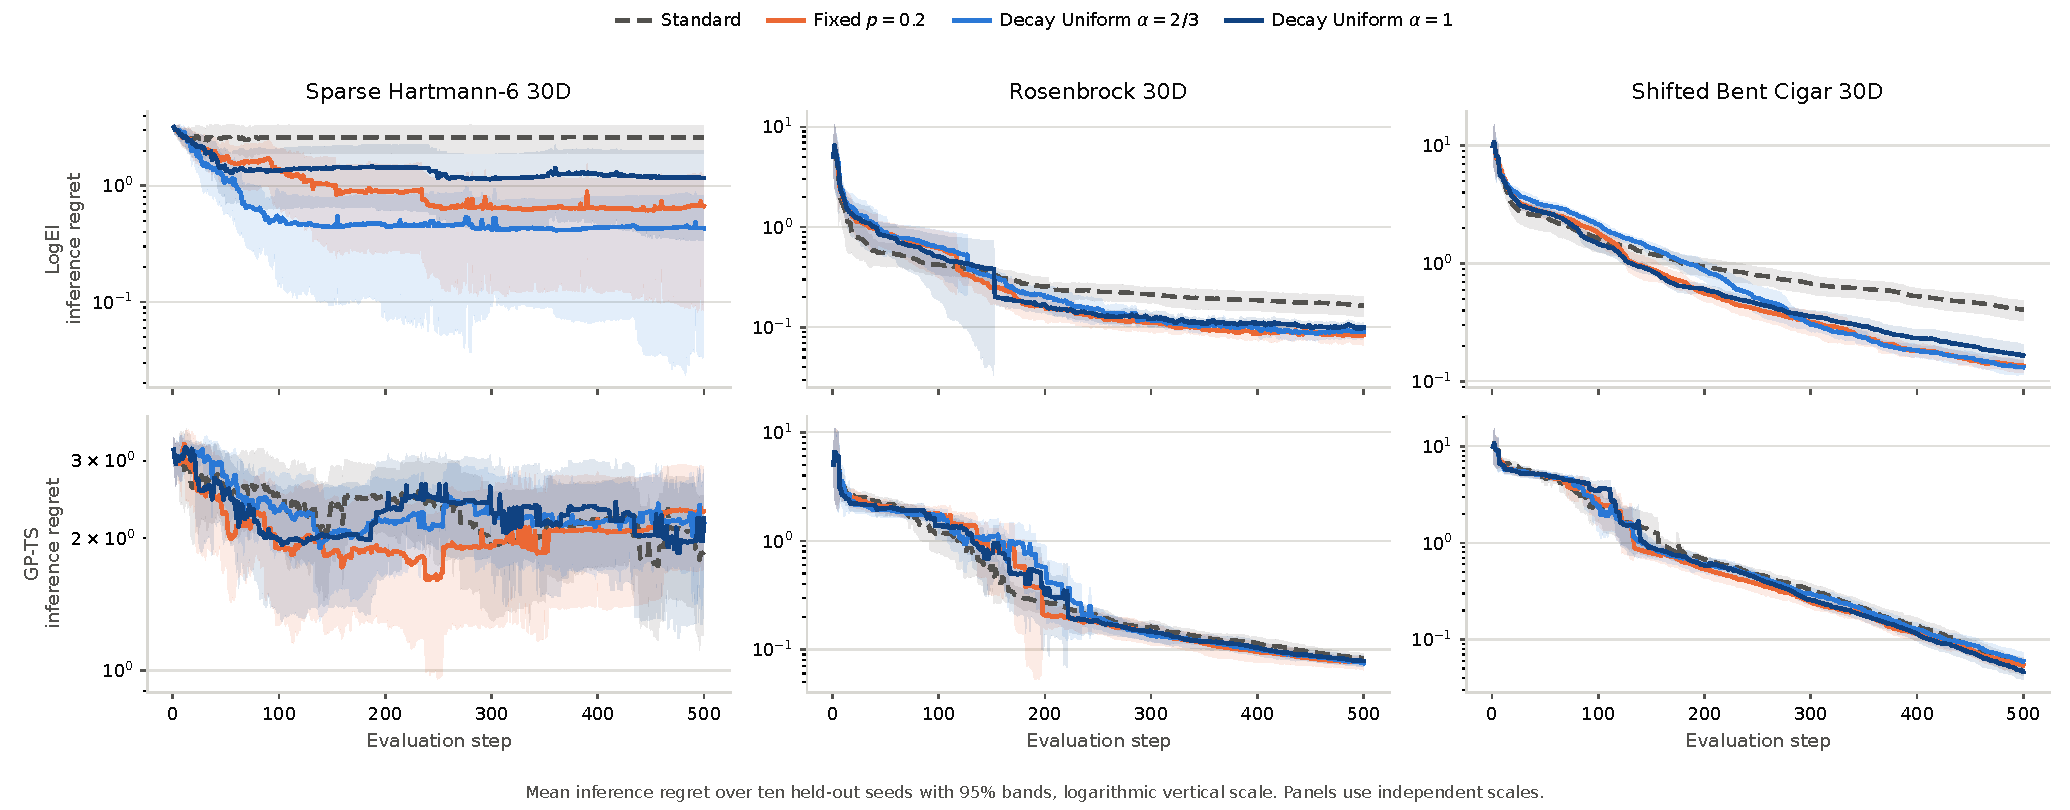
\includegraphics[width=\textwidth]{figures/fig_acquisition_30d_trajectories.pdf}
  \caption{Inference regret against evaluation step under LogEI (top) and
  GP-TS (bottom); lower is better.}
  \label{fig:trajectories}
\end{figure}

Under LogEI the gap opens early on Sparse Hartmann and holds for the rest of
the run; on Bent Cigar it opens near step 130 and widens to the end; on
Rosenbrock the PE arms are worse than Standard until about step 150. Under
GP-TS, Rosenbrock ends below Standard for the two slower decay schedules,
whereas Bent Cigar is mixed and Sparse Hartmann does not show a stable gain.

\subsection{Replication on unseen seeds}

\setup Sparse Hartmann and Rosenbrock were first run on five pilot seeds, then
on ten seeds disjoint from them. $\alpha=2/3$ is fixed in advance, not selected.

\begin{figure}[H]
  \centering
  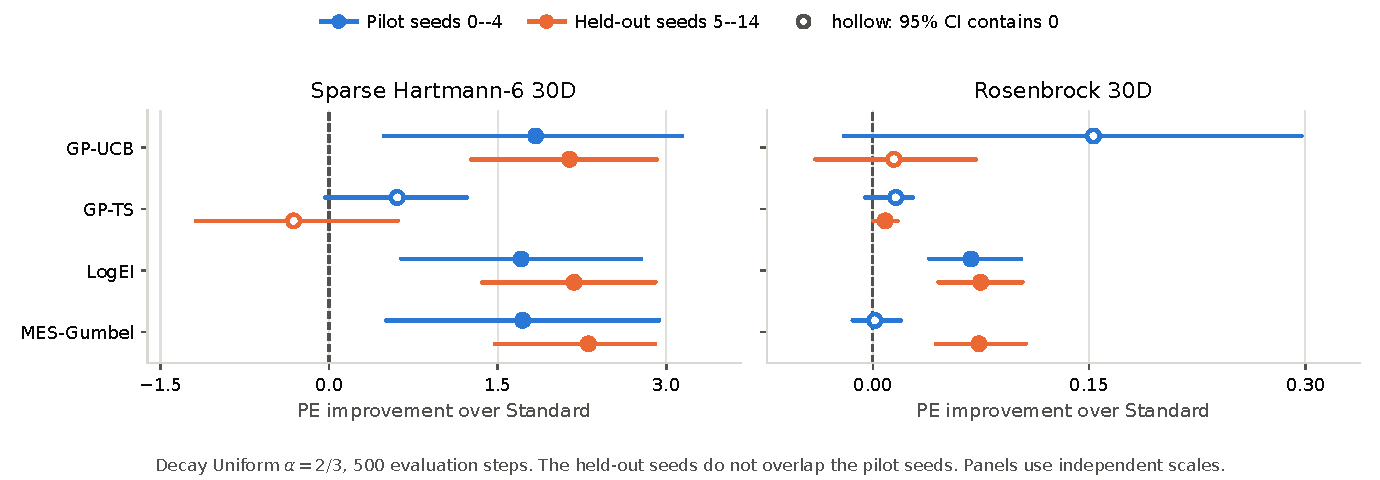
\includegraphics[width=0.667\textwidth]{figures/fig_acquisition_pilot_vs_heldout.pdf}
  \caption{Decay Uniform $\alpha=2/3$ on the pilot seeds and on the held-out
  seeds.}
  \label{fig:acqreplication}
\end{figure}

\begin{table}[H]
\centering
\small
\begin{tabular}{@{}llrlrrlr@{}}
\toprule
 & & \multicolumn{3}{c}{Pilot, seeds 0--4} & \multicolumn{3}{c}{Held-out, seeds 5--14} \\
\cmidrule(lr){3-5}\cmidrule(l){6-8}
Objective & Acquisition & Improv. & 95\% CI & W/L & Improv. & 95\% CI & W/L \\
\midrule
Sparse Hartmann-30 & GP-UCB & \pewin{1.838} & $[0.488, 3.141]$ & 4/1 & \pewin{2.140} & $[1.266, 2.916]$ & 9/1 \\
 & GP-TS & \pesoft{0.607} & $[-0.035, 1.228]$ & 4/1 & \stdsoft{-0.315} & $[-1.182, 0.610]$ & 4/6 \\
 & LogEI & \pewin{1.710} & $[0.644, 2.776]$ & 4/1 & \pewin{2.180} & $[1.362, 2.902]$ & 9/1 \\
 & MES-Gumbel & \pewin{1.722} & $[0.506, 2.937]$ & 4/1 & \pewin{2.307} & $[1.478, 2.900]$ & 9/1 \\
\addlinespace
Rosenbrock-30 & GP-UCB & \pesoft{0.1530} & $[-0.0202, 0.2973]$ & 4/1 & \pesoft{0.0145} & $[-0.0398, 0.0712]$ & 6/4 \\
 & GP-TS & \pesoft{0.0158} & $[-0.0055, 0.0274]$ & 4/1 & \pewin{0.0085} & $[0.0004, 0.0170]$ & 7/3 \\
 & LogEI & \pewin{0.0681} & $[0.0391, 0.1027]$ & 5/0 & \pewin{0.0747} & $[0.0455, 0.1036]$ & 10/0 \\
 & MES-Gumbel & \pesoft{0.0013} & $[-0.0140, 0.0191]$ & 3/2 & \pewin{0.0736} & $[0.0436, 0.1059]$ & 9/1 \\
\bottomrule
\end{tabular}

\caption{Pilot and held-out estimates for Decay Uniform $\alpha=2/3$.}
\label{tab:acqreplication}
\end{table}

\findings
\begin{itemize}
  \item The non-TS cells largely keep their earlier conclusion, and every one
        significant on the pilot seeds is significant again: Sparse Hartmann GP-UCB $1.838\to2.140$,
        LogEI $1.710\to2.180$, MES-Gumbel $1.722\to2.307$, Rosenbrock LogEI
        $0.0681\to0.0747$.
  \item Rosenbrock MES-Gumbel becomes significant only on the held-out seeds.
        With the replacement GP-TS, Sparse Hartmann flips from a positive
        pilot estimate to a negative held-out estimate, with both intervals
        containing zero. Rosenbrock keeps the positive direction and becomes
        significant on the held-out seeds ($0.0085$).
  \item An earlier pilot with sixty initial evaluations gave a different
        answer and is not pooled with these results. The conclusions above are
        for the $n_{\mathrm{initial}}=2$ protocol shown in
        Table~\ref{tab:scope}.
\end{itemize}

\section{Does the benefit appear across benchmarks?}
\label{sec:bench}

\setup Three functions that extend across dimension --- rotated shifted
mean-scaled Rastrigin, Rosenbrock, and shifted Ackley --- swept over seven
exponents at $d\in\{2,5,10,20,30\}$ under GP-UCB with Decay Uniform. Ackley uses
a deterministic interior shift at every dimension so the optimum is never
central. Each run has 400 BO steps after two initial evaluations, with five
paired seeds.

\begin{figure}[H]
  \centering
  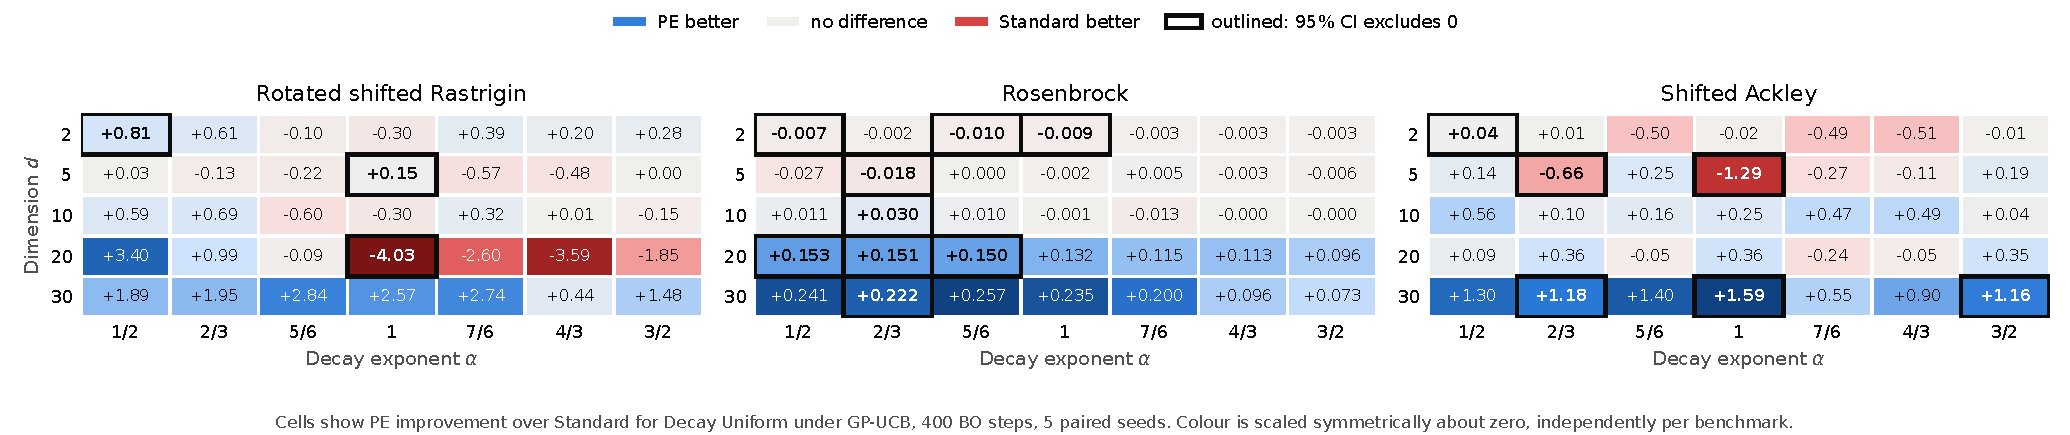
\includegraphics[width=\textwidth]{figures/fig_alpha_dimension_heatmap.pdf}
  \caption{Paired improvement for every dimension and exponent on the three
  scalable benchmarks.}
  \label{fig:threebench}
\end{figure}

\begin{table}[H]
\centering
\small
\begin{tabular}{@{}llrlrrrr@{}}
\toprule
Benchmark & $d$ & Standard & Best $\alpha$ & PE & Improv. & 95\% CI & W/L \\
\midrule
Rastrigin & $2$ & $1.114$ & $1/2$ & $0.301$ & \pewin{0.813} & $[0.503, 1.420]$ & 5/0 \\
 & $5$ & $1.482$ & $1$ & $1.333$ & \pewin{0.149} & $[0.018, 0.278]$ & 4/1 \\
 & $10$ & $6.880$ & $2/3$ & $6.192$ & \pesoft{0.688} & $[-4.413, 5.789]$ & 2/3 \\
 & $20$ & $6.367$ & $1/2$ & $2.972$ & \pesoft{3.396} & $[-0.801, 7.592]$ & 3/2 \\
 & $30$ & $9.183$ & $5/6$ & $6.347$ & \pesoft{2.836} & $[-0.624, 5.630]$ & 4/1 \\
\addlinespace
Rosenbrock & $2$ & $0.0027$ & $2/3$ & $0.0050$ & \stdsoft{-0.0023} & $[-0.0054, 0.0002]$ & 2/3 \\
 & $5$ & $0.0231$ & $7/6$ & $0.0178$ & \pesoft{0.0053} & $[-0.0065, 0.0148]$ & 4/1 \\
 & $10$ & $0.0895$ & $2/3$ & $0.0596$ & \pewin{0.0299} & $[0.0075, 0.0559]$ & 4/1 \\
 & $20$ & $0.2815$ & $1/2$ & $0.1289$ & \pewin{0.1526} & $[0.0273, 0.3459]$ & 4/1 \\
 & $30$ & $0.4435$ & $5/6$ & $0.1864$ & \pesoft{0.2571} & $[-0.0154, 0.5948]$ & 4/1 \\
\addlinespace
Shifted Ackley & $2$ & $0.0531$ & $1/2$ & $0.0175$ & \pewin{0.0356} & $[0.0086, 0.0591]$ & 4/1 \\
 & $5$ & $1.161$ & $5/6$ & $0.908$ & \pesoft{0.253} & $[-0.843, 1.166]$ & 3/2 \\
 & $10$ & $2.426$ & $1/2$ & $1.870$ & \pesoft{0.557} & $[-0.660, 1.718]$ & 3/2 \\
 & $20$ & $3.027$ & $2/3$ & $2.667$ & \pesoft{0.360} & $[-0.253, 1.076]$ & 3/2 \\
 & $30$ & $5.167$ & $1$ & $3.581$ & \pewin{1.586} & $[0.311, 2.995]$ & 4/1 \\
\bottomrule
\end{tabular}

\caption{The exponent with the largest mean improvement at each benchmark and
dimension.}
\label{tab:bestalpha}
\end{table}

\findings
\begin{itemize}
  \item All three benchmarks contain significant cells in both directions.
  \item Rosenbrock moves with dimension: three exponents at 2D and $\alpha=2/3$
        at 5D favor Standard, then PE gains at 10D $\alpha=2/3$ $(0.0299$
        $[0.0075, 0.0559])$, at 20D for $\alpha=1/2,2/3,5/6$ $(0.150$ to
        $0.153)$, and at 30D $\alpha=2/3$ $(0.2218$ $[0.0022, 0.5016])$.
  \item Ackley gains at 2D $\alpha=1/2$ $(0.0356$ $[0.0086, 0.0591])$ and at 30D
        for $\alpha=2/3,1,3/2$ $(1.16$ to $1.59)$, but loses at 5D for
        $\alpha=2/3$ and $\alpha=1$.
  \item Rastrigin gains at 2D $\alpha=1/2$ $(0.813$ $[0.503, 1.420]$, 5/5 seeds)
        and 5D $\alpha=1$ $(0.149)$, and loses at 20D $\alpha=1$ $(-4.03)$. Its
        large 20D and 30D positive means have intervals containing zero.
\end{itemize}

\begin{figure}[H]
  \centering
  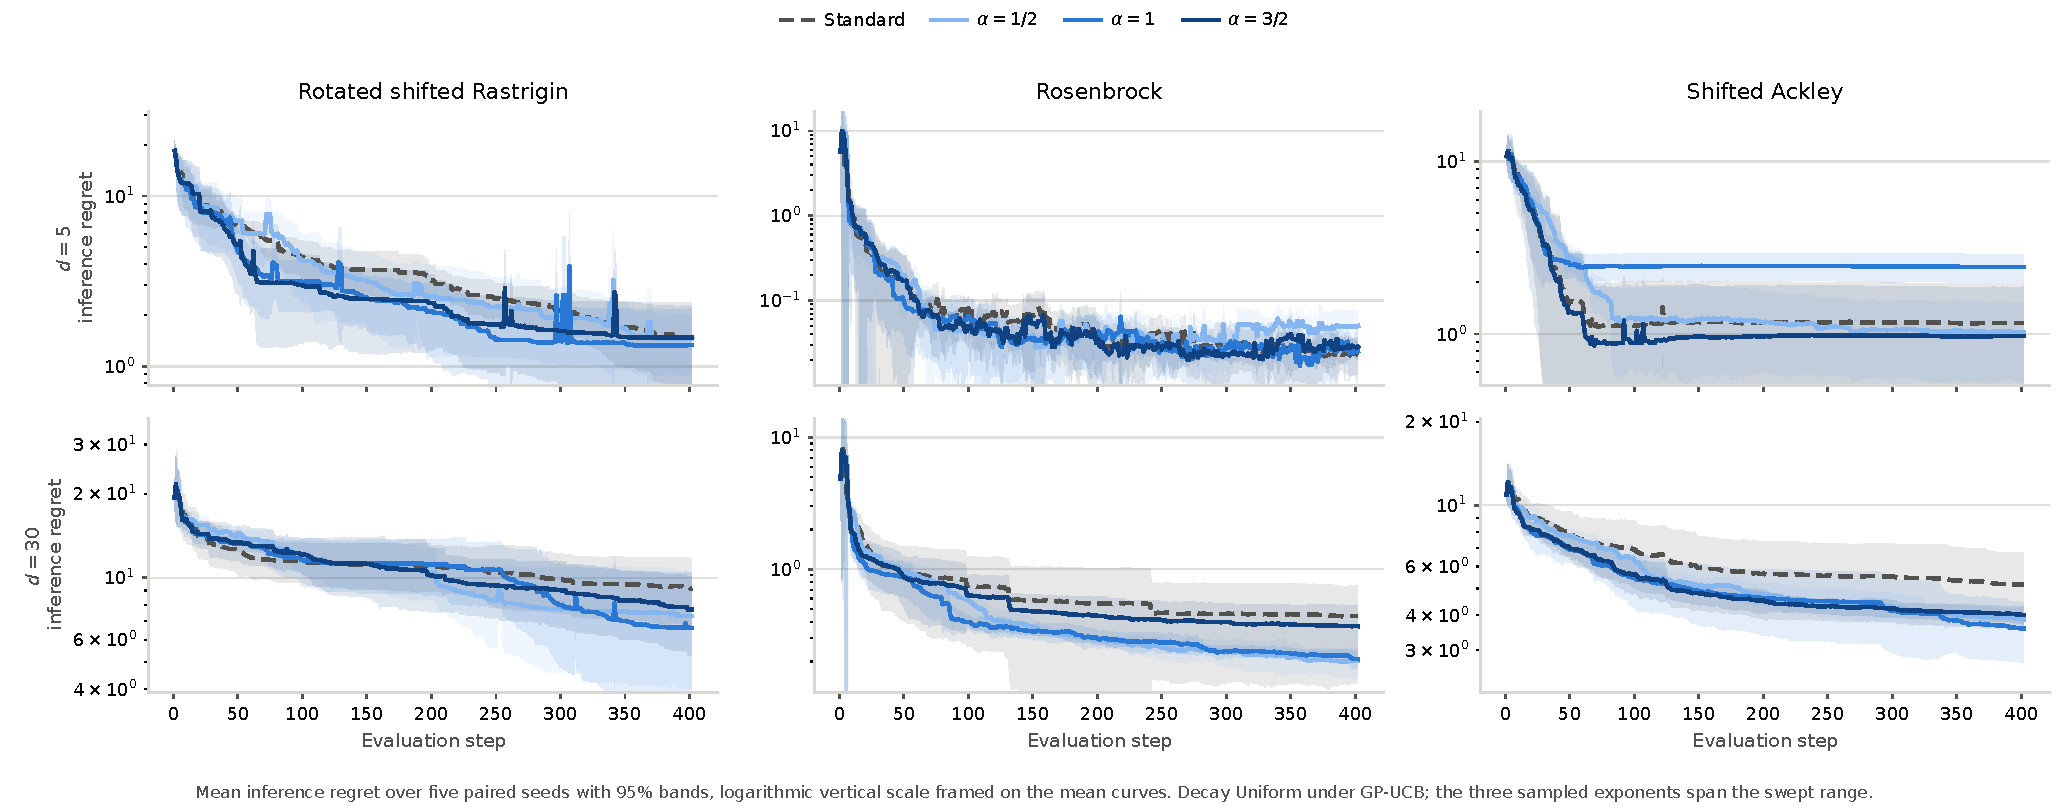
\includegraphics[width=\textwidth]{figures/fig_alpha_dimension_trajectories.pdf}
  \caption{Inference regret against evaluation step at $d=5$ and $d=30$;
  lower is better.}
  \label{fig:benchtraj}
\end{figure}

At $d=5$ the PE and Standard curves stay inside each other's bands on Rastrigin and
Rosenbrock, and on Ackley the $\alpha=1$ arm stalls above Standard for the whole
run. At $d=30$ the mean PE curves move below Standard inside the first hundred
steps and keep the gap to the end on all three benchmarks. The endpoint pattern
is therefore not created only by the final few evaluations, although several
endpoint intervals still contain zero.

\section{Is the best exponent a function of the dimension?}
\label{sec:dimalpha}

\findings
\begin{itemize}
  \item Reading the best exponent down Table~\ref{tab:bestalpha} gives
        $1/2,\allowbreak 1,\allowbreak 2/3,\allowbreak 1/2,\allowbreak 5/6$ for
        Rastrigin, $2/3,\allowbreak 7/6,\allowbreak 2/3,\allowbreak
        1/2,\allowbreak 5/6$ for Rosenbrock, and $1/2,\allowbreak
        5/6,\allowbreak 1/2,\allowbreak 2/3,\allowbreak 1$ for Ackley. The
        values cluster in $[1/2, 1]$ and are not ordered by dimension in any benchmark. No
        dimension has one winner shared by all three benchmarks. Rastrigin
        and Rosenbrock agree at 10D, 20D, and 30D, while Ackley selects a
        different exponent in those dimensions.
  \item On Rosenbrock and Ackley the largest gains appear at higher dimensions,
        while the best exponent is not monotone in dimension. Every significant
        high-dimensional cell on those two
        benchmarks lies in $\alpha\in[1/2,1]$, except Ackley 30D at
        $\alpha=3/2$.
  \item The largest mean is not always the significant cell: at 30D Rosenbrock
        the best mean is $\alpha=5/6$ $(0.2571$ $[-0.0154, 0.5948])$ while the
        significant cell is $\alpha=2/3$.
  \item Rows of Figure~\ref{fig:threebench} look flat in $\alpha$ wherever PE
        helps, but that reading comes from five-seed sweeps. On ten held-out
        seeds (Section~\ref{sec:acq}) the same range is not flat: $\alpha=1/2$
        beats $\alpha=2/3$ by a factor of ten on Bent Cigar under GP-UCB.
  \item Figure~\ref{fig:benchtraj} shows this at the trajectory level: at $d=30$
        the $\alpha=1/2$ and $\alpha=1$ curves are close to indistinguishable on
        all three benchmarks, while $\alpha=3/2$ sits between them and Standard
        and keeps part of the gain $(+1.48$ against $+2.57$ on Rastrigin,
        $+0.073$ against $+0.235$ on Rosenbrock, $+1.16$ against $+1.59$ on
        Ackley$)$. The flatness holds inside $[1/2,1]$, not across the whole
        sweep.
\end{itemize}

A separate Rastrigin pilot compared seven Uniform and seven
maximum-posterior-variance (MVR) decay schedules, plus Standard, using
$n_{\mathrm{initial}}=2d$. Its 375 runs give the same qualitative answer: the
preferred exponent is no more predictable from dimension under MVR, and the
two point-selection rules can disagree in direction at the same dimension.

\section{Can the exponent be chosen in practice?}
\label{sec:choice}

\setup The procedure tested is: sweep $\alpha$ on five seeds, keep the
per-dimension winner, then evaluate that winner on seeds not used for the
selection. The winners from the Rastrigin sweep were rerun against Standard on
fifteen disjoint seeds under identical conditions.

\begin{figure}[H]
  \centering
  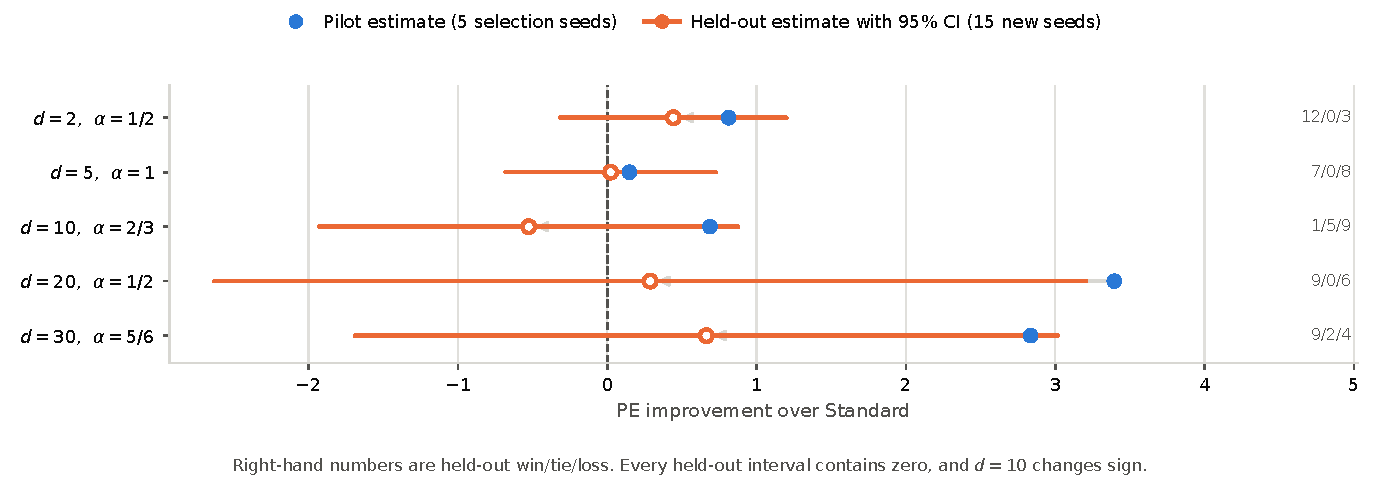
\includegraphics[width=0.667\textwidth]{figures/fig_alpha_selection_heldout.pdf}
  \caption{Pilot estimate and held-out estimate for the selected exponent at
  each dimension.}
  \label{fig:confirmation}
\end{figure}

\begin{table}[H]
\centering
\small
\begin{tabular}{@{}llrrrr@{}}
\toprule
$d$ & Selected $\alpha$ & Pilot improvement & Held-out improvement & 95\% CI & W/T/L \\
\midrule
$2$ & $1/2$ & $0.81$ & \pesoft{0.44} & $[-0.31, 1.20]$ & 12/0/3 \\
$5$ & $1$ & $0.15$ & \pesoft{0.02} & $[-0.68, 0.73]$ & 7/0/8 \\
$10$ & $2/3$ & $0.69$ & \stdsoft{-0.53} & $[-1.93, 0.88]$ & 1/5/9 \\
$20$ & $1/2$ & $3.40$ & \pesoft{0.29} & $[-2.63, 3.21]$ & 9/0/6 \\
$30$ & $5/6$ & $2.84$ & \pesoft{0.66} & $[-1.69, 3.02]$ & 9/2/4 \\
\bottomrule
\end{tabular}

\caption{Pilot versus held-out improvement for the selected exponent.}
\label{tab:confirmation}
\end{table}

\findings
\begin{itemize}
  \item None of the five selections replicates: every held-out interval contains
        zero and the effects shrink three- to twelvefold, with 20D falling from
        $3.40$ to $0.29$ and 30D from $2.84$ to $0.66$.
  \item At 10D the sign reverses, from $0.69$ to $-0.53$ with 1 win, 5 ties, and
        9 losses. Win counts still favor PE at 2D, 20D, and 30D.
\end{itemize}

\subsection{Increasing the selection set from five to twenty seeds}

\setup The sweep was extended to 35 seeds. The per-dimension winner is chosen on
seeds 0--19 and evaluated on seeds 20--34, which were not used for selection.

\begin{figure}[H]
  \centering
  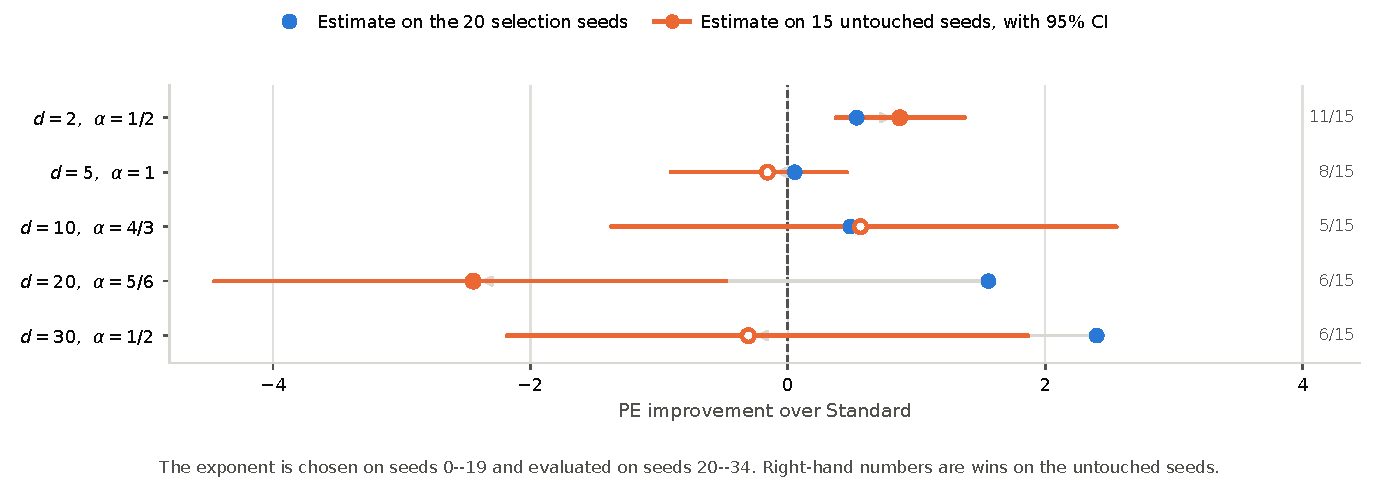
\includegraphics[width=0.667\textwidth]{figures/fig_alpha_selection_fresh_seeds.pdf}
  \caption{Estimate on the twenty selection seeds and on the fifteen untouched
  seeds, for the exponent chosen at each dimension.}
  \label{fig:freshselection}
\end{figure}

\begin{table}[H]
\centering
\small
\begin{tabular}{@{}llrrlrrr@{}}
\toprule
 & \multicolumn{4}{c}{Exponent chosen on seeds 0--19} & \multicolumn{2}{c}{No selection, $\alpha=1/2$} \\
\cmidrule(lr){2-6}\cmidrule(l){7-8}
$d$ & Pick & Train & Test & Test 95\% CI & Wins & Test & Wins \\
\midrule
$2$ & $1/2$ & $0.536$ & \pewin{0.869} & $[0.375, 1.370]$ & 11/15 & \pewin{0.869} & 11/15 \\
$5$ & $1$ & $0.054$ & \stdsoft{-0.158} & $[-0.920, 0.456]$ & 8/15 & \stdwin{-0.723} & 4/15 \\
$10$ & $4/3$ & $0.487$ & \pesoft{0.565} & $[-1.404, 2.520]$ & 5/15 & \pesoft{1.084} & 10/15 \\
$20$ & $5/6$ & $1.559$ & \stdwin{-2.445} & $[-4.508, -0.503]$ & 6/15 & \stdsoft{-1.049} & 9/15 \\
$30$ & $1/2$ & $2.401$ & \stdsoft{-0.307} & $[-2.192, 1.850]$ & 6/15 & \stdsoft{-0.307} & 6/15 \\
\bottomrule
\end{tabular}

\caption{The selected exponent and a pre-fixed $\alpha=1/2$, both scored on
seeds 20--34.}
\label{tab:selectionfresh}
\end{table}

\findings
\begin{itemize}
  \item Only $d=2$ replicates, at $0.869$ $[0.386, 1.382]$. At $d=20$ the
        selected $\alpha=5/6$ moves from $+1.559$ on the selection seeds to
        $-2.445$ $[-4.495, -0.473]$ on the untouched ones, a reversal that is
        itself significant.
  \item Not selecting does better. Fixing $\alpha=1/2$ scores $-0.025$ averaged
        over the five dimensions against $-0.295$ for the selection rule, though
        it is significantly worse than Standard at $d=5$.
  \item Averaged over 200 random train/test splits inside seeds 0--19, fixing
        $\alpha=1/2$ returns $+0.592 \pm 0.179$ and is positive in 100\% of
        splits, while the best selection rule tested --- pick the exponent with
        the highest win rate --- returns $+0.466 \pm 0.228$ in 96\%. Picking by
        mean, median, lower confidence bound or a smoothed argmax all do worse.
        A post-hoc oracle would return $+1.040$. Thus the grid contains better
        choices, but the tested selection rules do not identify them reliably.
\end{itemize}

\begin{table}[H]
\centering
\small
\begin{tabular}{@{}lrrrlr@{}}
\toprule
$d$ & Seeds 0--19 & Seeds 20--34 & All 35 & 95\% CI & W/L \\
\midrule
$2$ & $0.536$ & $0.869$ & \pewin{0.679} & $[0.319, 1.062]$ & 28/35 \\
$5$ & $-0.294$ & $-0.723$ & \stdwin{-0.478} & $[-0.834, -0.127]$ & 14/35 \\
$10$ & $-0.592$ & $1.084$ & \pesoft{0.126} & $[-1.040, 1.352]$ & 16/35 \\
$20$ & $1.065$ & $-1.049$ & \pesoft{0.159} & $[-1.651, 1.962]$ & 21/35 \\
$30$ & $2.401$ & $-0.307$ & \pesoft{1.240} & $[-0.125, 2.627]$ & 22/35 \\
\bottomrule
\end{tabular}

\caption{The same cell, $\alpha=1/2$, estimated on two disjoint seed blocks.}
\label{tab:seedblocks}
\end{table}

Table~\ref{tab:seedblocks} explains why. At $d=30$ the same policy measures
$+2.401$ on seeds 0--19 and $-0.307$ on seeds 20--34. Rastrigin at 400 BO steps
carries enough seed variance that a twenty-seed block estimate moves by more than
the effect being measured, so any per-dimension number from this sweep should be
read as specific to its seed block.

The simple run-conditioned rule tested here is also insufficient. A 40-step
Standard prefix has no consistent association with the later PE outcome: the
Spearman correlation
between the prefix improvement rate and the eventual gain at $\alpha=1/2$ is
$-0.23, 0.11, 0.07, 0.33, -0.08$ across the five dimensions, and the correlation
with the seed's own best exponent never exceeds $0.26$ in magnitude. The per-seed
best exponent is not concentrated either: at $d=5$ the modal exponent wins on 4
of 20 seeds and at $d=30$ on 5 of 20, so there is no stable target to predict.

\section{Lunar Lander controller tuning}
\label{sec:external}

\setup This is the 12-parameter Lunar Lander controller problem used by TuRBO.
One evaluation flies the controller on 50 fixed terrains and uses their average
return. We ran 30 seeds. Policies in the same seed share the terrains and the 24
initial Sobol points, so the comparison is paired. Each run has 400 evaluations.

The GP uses a Mat\'ern kernel, fixes signal variance to $1$, and learns only the
lengthscales. The completed results use GP-UCB, GP-TS, LogEI, and MES-Gumbel
with five policies:
Standard, decay $\alpha=1/2,2/3,1$, and Fixed $p=0.2$.
The GP-TS row is the completed 150-trial replacement using
$\beta_t=\log(t+1)$ and the increasing Sobol discretization described above;
the previous fixed-$\beta$ result is not used.

A controller is counted as solved when its average return is at least 200. We
report return directly because 200 is a success threshold, not the true optimum.

\begin{figure}[H]
  \centering
  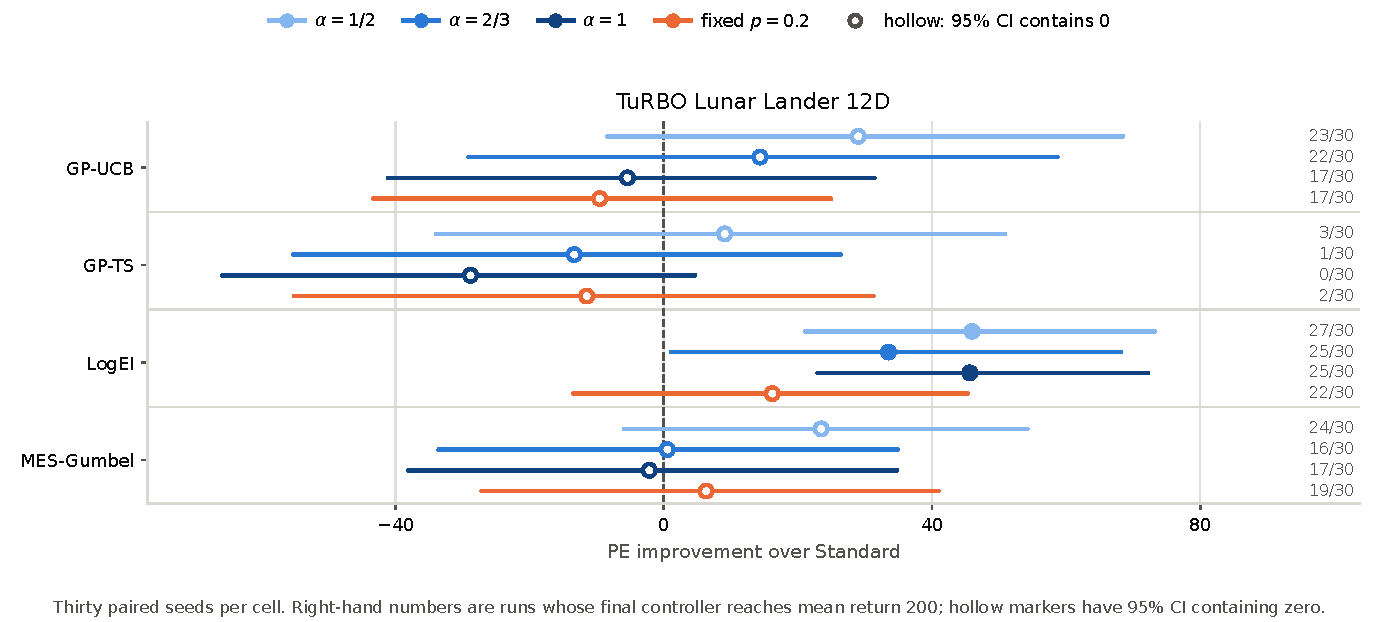
\includegraphics[width=0.667\textwidth]{figures/fig_lunar_returns.pdf}
  \caption{How much each PE policy changes the final return. Positive values
  favor PE. Right-hand numbers are solved runs out of 30.}
  \label{fig:lunarreturns}
\end{figure}

\begin{table}[H]
\centering
\small
\begin{tabular}{@{}lrrrrr@{}}
\toprule
Policy & Mean return & Improvement & 95\% CI & Solved runs & PE queries \\
\midrule
Standard & $215.8$ & -- & -- & 21/30 & $0.0$ \\
$\alpha=1/2$ & $261.8$ & \pewin{46.0} & $[21.2, 73.4]$ & 27/30 & $155.3$ \\
$\alpha=2/3$ & $249.3$ & \pewin{33.5} & $[1.4, 68.0]$ & 25/30 & $71.2$ \\
$\alpha=1$ & $261.5$ & \pewin{45.6} & $[23.2, 71.9]$ & 25/30 & $17.4$ \\
fixed $p=0.2$ & $232.0$ & \pesoft{16.2} & $[-12.8, 44.9]$ & 22/30 & $73.3$ \\
\bottomrule
\end{tabular}

\caption{LogEI results. Each improvement is compared with Standard using the
same 30 seeds. PE queries exclude the 24 initial evaluations.}
\label{tab:lunarlogei}
\end{table}

\findings
\begin{itemize}
  \item LogEI is the clearest case. Standard scores $215.8$. Decay
        $\alpha=1/2$ scores $261.8$ $(+46.0)$, and $\alpha=1$ scores $261.5$
        $(+45.6)$. Both confidence intervals exclude zero.
  \item With LogEI, solved runs increase from 21/30 to 27/30 at
        $\alpha=1/2$. A crash gives roughly $-100$, so a 50-terrain average over
        200 means the controller lands reliably.
  \item At $\alpha=1/2$, GP-UCB improves by $+29.0$ and MES-Gumbel by $+23.5$.
        Their confidence intervals still include zero.
  \item Under the replacement GP-TS, $\alpha=1/2$ changes mean return by
        $+9.1$ with a 95\% interval of $[-32.8,+50.1]$. The solved count is
        4/30 for Standard and 3/30 for PE, so this setting gives no clear
        evidence of a GP-TS gain on Lunar.
\end{itemize}

\subsection{When PE is used matters}

\begin{table}[H]
\centering
\small
\begin{tabular}{@{}lrrrr@{}}
\toprule
Decay policy & Mean PE queries & Improvement over Fixed & 95\% CI & W/L \\
\midrule
$\alpha=1/2$ & $155.3$ & \pewin{29.8} & $[6.6, 54.9]$ & 19/11 \\
$\alpha=2/3$ & $71.2$ & \pesoft{17.3} & $[-17.2, 50.6]$ & 17/13 \\
$\alpha=1$ & $17.4$ & \pewin{29.4} & $[9.1, 52.2]$ & 19/11 \\
\bottomrule
\end{tabular}

\caption{Decay schedules compared directly with Fixed $p=0.2$ under LogEI.}
\label{tab:lunarschedule}
\end{table}

Decay $\alpha=1$ beats Fixed $p=0.2$ by $+29.4$ $[+9.1,+52.2]$. It uses only
17.4 random queries on average, while Fixed uses 73.3. Therefore, the gain is not
simply from using more random queries. Using PE early and then returning to
LogEI appears better than spreading random queries across the whole run. A
matched-count experiment is still needed to confirm this point.

\subsection{The improvement transfers to unseen terrains}

The results above score each controller on the 50 episode seeds used during its
own BO run. To check whether those results are specific to that set, we took all
150 final LogEI controllers (30 BO seeds and five policies) and evaluated every
one on the same 200 new episode seeds. None of these seeds appears among the
1{,}500 seeds used during optimisation. This is a separate test of the final
controllers; BO was not run again. In total, the check contains 30{,}000 new
rollouts.

\begin{figure}[H]
  \centering
  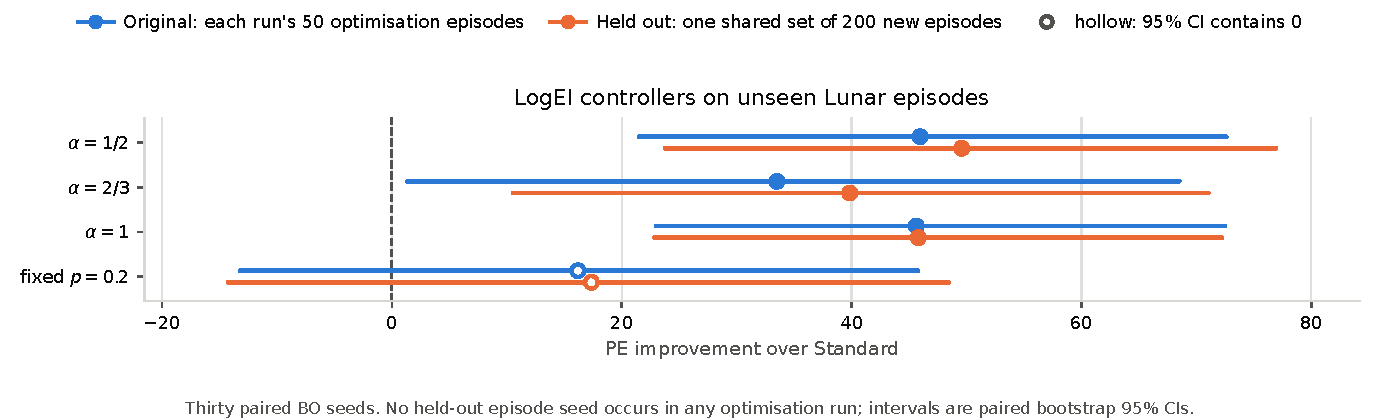
\includegraphics[width=0.667\textwidth]{figures/fig_lunar_heldout_generalization.pdf}
  \caption{The LogEI improvement on each run's original 50 episodes and on a
  shared set of 200 unseen episodes. The two estimates are nearly unchanged.}
  \label{fig:lunarheldout}
\end{figure}

\begin{table}[H]
\centering
\scriptsize
\begin{tabular}{@{}lrrrrr@{}}
\toprule
Policy & Mean return & Gain vs. Standard (95\% CI) & Episodes $\geq 200$ & Bottom 10\% & Solved \\
\midrule
Standard & 209.9 & -- & 73.1\% & 48.8 & 20/30 \\
$\alpha=1/2$ & \textbf{259.5} & \pewin{49.6} $[23.7, 76.9]$ & \textbf{91.4\%} & \textbf{124.7} & \textbf{27/30} \\
$\alpha=2/3$ & 249.8 & \pewin{39.8} $[10.6, 71.0]$ & 87.5\% & 114.2 & 25/30 \\
$\alpha=1$ & 255.7 & \pewin{45.8} $[22.8, 72.2]$ & 89.0\% & 113.5 & 25/30 \\
Fixed $p=0.2$ & 227.3 & \pesoft{17.4} $[-14.3, 48.4]$ & 78.8\% & 57.4 & 22/30 \\
\bottomrule
\end{tabular}

\caption{Performance on 200 unseen episodes. ``Episodes $\geq 200$'' is the
fraction of individual episodes whose return reaches 200. ``Bottom 10\%'' is
the mean of each controller's 20 lowest returns. A controller is solved when
its mean over all 200 episodes reaches 200.}
\label{tab:lunarheldout}
\end{table}

All three decay schedules remain better than Standard: their paired
mean-return confidence intervals stay above zero. The largest average result is
$\alpha=1/2$: mean return rises from $209.9$ to $259.5$, the fraction of
episodes reaching 200 rises from $73.1\%$ to $91.4\%$, and solved controllers
rise from 20/30 to 27/30. Its bottom-10\% return also rises from $48.8$ to
$124.7$, so the gain is not limited to easy terrains. The original and held-out
improvements are $+46.0$ and $+49.6$, respectively. Fixed $p=0.2$ remains
uncertain, while decay $\alpha=1/2$ beats it by $+32.2$ $[+6.9,+59.9]$ on the
new episodes. This is strong evidence against the explanation that PE only
found controllers specialised to the 50 episodes used during optimisation.

\begin{figure}[H]
  \centering
  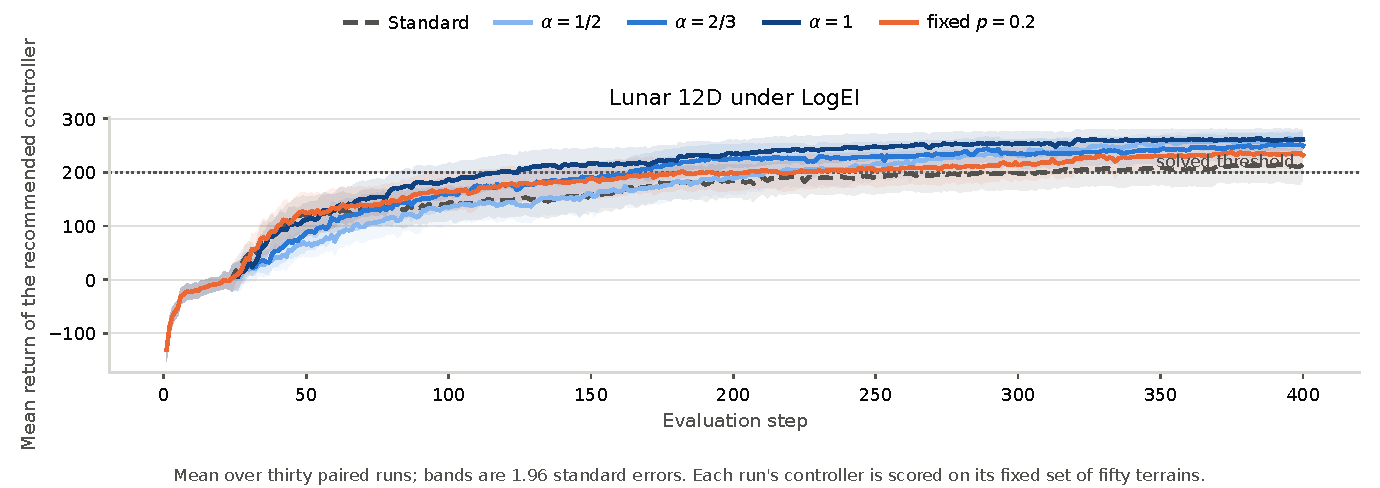
\includegraphics[width=0.667\textwidth]{figures/fig_lunar_logei_trajectory.pdf}
  \caption{Mean return of the currently recommended controller as LogEI
  accumulates evaluations. The dotted line is the solved threshold of 200.}
  \label{fig:lunartrajectory}
\end{figure}

\section{Hyperparameter optimisation}
\label{sec:hpo}

As a first transfer test outside analytic functions and simulation control, we
ran six scikit-learn model-tuning tasks with GP-UCB and LogEI. The confirmation
uses 20 paired seeds per cell, 100 evaluations, and the same fixed unit signal
variance. Across 36 acquisition--task--PE comparisons, no PE policy gives a
significant held-out test-loss improvement over Standard. The result is useful
as a negative transfer check: the current evidence does not support claiming
that PE helps every HPO problem.

The higher-dimensional YAHPO study uses GP-UCB, LogEI, theory-aligned GP-TS,
and MES-Gumbel with Standard, decay $\alpha=1/2$, decay $\alpha=1$, and Fixed
$p=0.2$. Every dimension uses ten initial points and thirty paired confirmation
seeds. The completed 14D stage covers three XGBoost tasks and 120 evaluations,
for 1,440 audited trials. The completed 28D stage covers two \texttt{iaml\_super}
tasks and 200 evaluations, for 960 audited trials.

Because YAHPO reports validation log loss, its improvement is Standard loss
minus PE loss. Figure~\ref{fig:yahpo14} shows the paired mean and bootstrap
95\% interval under the same positive-is-better convention used elsewhere.

\begin{figure}[H]
  \centering
  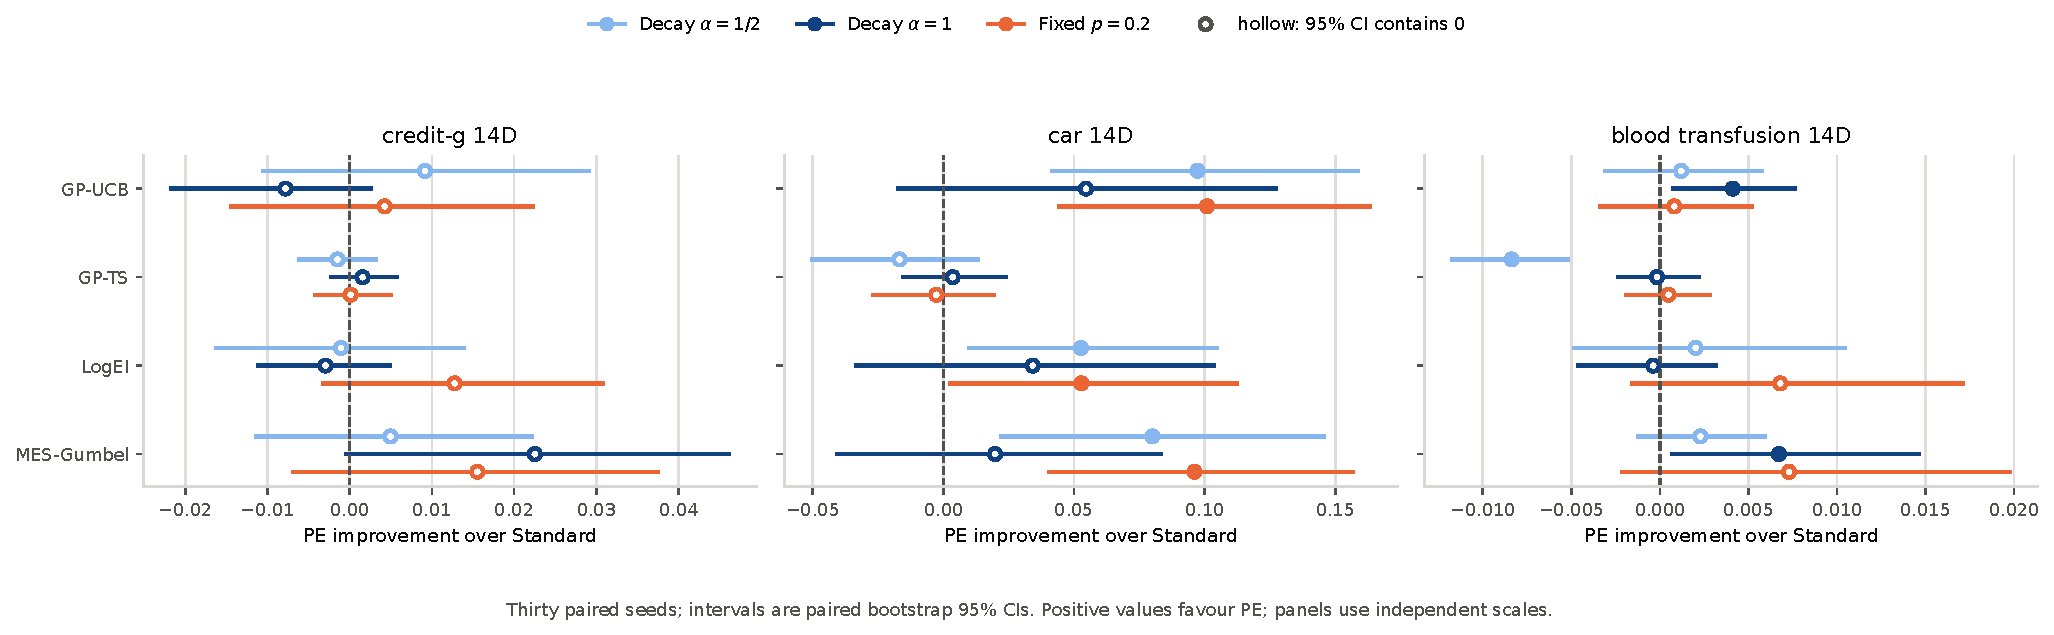
\includegraphics[width=\textwidth]{figures/fig_yahpo_14d_endpoint_improvement.pdf}
  \caption{Endpoint improvement over Standard on the completed 14D YAHPO
  tasks. Filled markers have paired 95\% intervals excluding zero; hollow
  markers have intervals containing zero.}
  \label{fig:yahpo14}
\end{figure}

\begin{table}[H]
\centering
\scriptsize
\begin{tabular}{@{}llrrr@{}}
\toprule
Dataset & Acquisition & $\alpha=1/2$ & $\alpha=1$ & Fixed $p=0.2$ \\
\midrule
credit-g & GP-UCB & \pesoft{+0.0092} & \stdsoft{-0.0078} & \pesoft{+0.0043} \\
 & GP-TS & \stdsoft{-0.0015} & \pesoft{+0.0016} & \pesoft{+0.0001} \\
 & LogEI & \stdsoft{-0.0010} & \stdsoft{-0.0029} & \pesoft{+0.0128} \\
 & MES-G & \pesoft{+0.0050} & \pesoft{+0.0225} & \pesoft{+0.0155} \\
\addlinespace
car & GP-UCB & \pewin{+0.0973} & \pesoft{+0.0546} & \pewin{+0.1009} \\
 & GP-TS & \stdsoft{-0.0167} & \pesoft{+0.0036} & \stdsoft{-0.0027} \\
 & LogEI & \pewin{+0.0527} & \pesoft{+0.0343} & \pewin{+0.0529} \\
 & MES-G & \pewin{+0.0800} & \pesoft{+0.0198} & \pewin{+0.0961} \\
\addlinespace
blood transfusion & GP-UCB & \pesoft{+0.0012} & \pewin{+0.0041} & \pesoft{+0.0008} \\
 & GP-TS & \stdwin{-0.0084} & \stdsoft{-0.0002} & \pesoft{+0.0005} \\
 & LogEI & \pesoft{+0.0020} & \stdsoft{-0.0004} & \pesoft{+0.0068} \\
 & MES-G & \pesoft{+0.0023} & \pewin{+0.0067} & \pesoft{+0.0073} \\
\bottomrule
\end{tabular}

\caption{Mean endpoint improvement over Standard in 14D YAHPO. Positive values
favor PE. Deep, bold cells have paired 95\% intervals excluding zero; complete
intervals and win/tie/loss counts are included in the public result CSV.}
\label{tab:yahpo14}
\end{table}

Across the 24 decay-policy comparisons, 5 improve significantly, 1 is
significantly worse, and 18 are inconclusive. The clearest pattern is on
\texttt{car}: $\alpha=1/2$ improves LogEI by $0.0527$
$[0.0100,0.1045]$, MES-Gumbel by $0.0800$ $[0.0224,0.1455]$, and GP-UCB by
$0.0973$ $[0.0418,0.1584]$. The median is not uniformly improved; the mean gain
comes mainly from reducing the high-loss tail. On \texttt{blood transfusion},
$\alpha=1$ improves MES-Gumbel and GP-UCB by $0.0067$ and $0.0041$,
respectively. No comparison is conclusive on \texttt{credit-g}. GP-TS shows no
reliable gain and is worse with $\alpha=1/2$ on \texttt{blood transfusion} by
$0.0084$ $[0.0052,0.0117]$. Finally, Fixed $p=0.2$ also improves UCB, LogEI,
and MES-Gumbel on \texttt{car}; this stage supports problem-dependent explicit
exploration, but does not establish that decay always beats a fixed rate.

Figure~\ref{fig:yahpo28} and Table~\ref{tab:yahpo28} summarize the completed
28D stage under the same convention.

\begin{figure}[H]
  \centering
  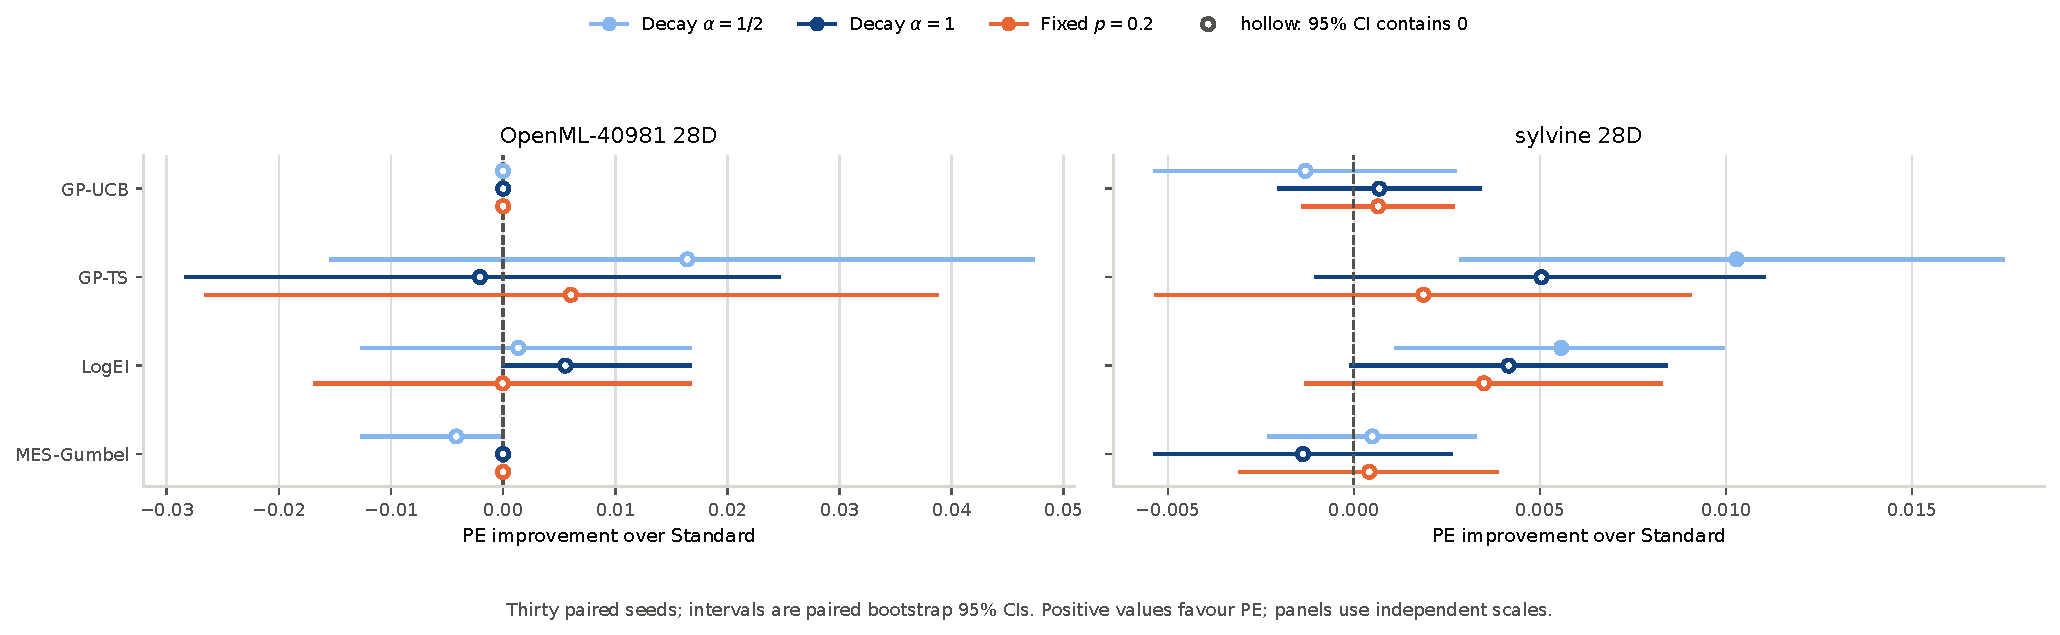
\includegraphics[width=\textwidth]{figures/fig_yahpo_28d_endpoint_improvement.pdf}
  \caption{Endpoint improvement over Standard on the completed 28D YAHPO
  tasks. Filled markers have paired 95\% intervals excluding zero; hollow
  markers have intervals containing zero.}
  \label{fig:yahpo28}
\end{figure}

\begin{table}[H]
\centering
\scriptsize
\begin{tabular}{@{}llrrr@{}}
\toprule
Dataset & Acquisition & $\alpha=1/2$ & $\alpha=1$ & Fixed $p=0.2$ \\
\midrule
OpenML-40981 & GP-UCB & $0.0000$ & $0.0000$ & $0.0000$ \\
 & GP-TS & \pesoft{+0.0164} & \stdsoft{-0.0021} & \pesoft{+0.0060} \\
 & LogEI & \pesoft{+0.0014} & \pesoft{+0.0056} & $0.0000$ \\
 & MES-G & \stdsoft{-0.0042} & $0.0000$ & $0.0000$ \\
\addlinespace
sylvine & GP-UCB & \stdsoft{-0.0013} & \pesoft{+0.0007} & \pesoft{+0.0007} \\
 & GP-TS & \pewin{+0.0103} & \pesoft{+0.0050} & \pesoft{+0.0019} \\
 & LogEI & \pewin{+0.0056} & \pesoft{+0.0042} & \pesoft{+0.0035} \\
 & MES-G & \pesoft{+0.0005} & \stdsoft{-0.0014} & \pesoft{+0.0004} \\
\bottomrule
\end{tabular}

\caption{Mean endpoint improvement over Standard in 28D YAHPO. Positive values
favor PE. Deep, bold cells have paired 95\% intervals excluding zero.}
\label{tab:yahpo28}
\end{table}

Across the 16 decay-policy comparisons, 2 improve significantly, none is
significantly worse, and 14 are inconclusive. Both clear gains occur on
\texttt{sylvine} with $\alpha=1/2$: LogEI improves by $0.0056$
$[0.0012,0.0099]$ and GP-TS by $0.0103$ $[0.0029,0.0174]$. GP-TS wins 21 of
30 paired seeds. No comparison is conclusive on \texttt{OpenML-40981}, where
many policies reach the same endpoint, and all Fixed $p=0.2$ comparisons are
inconclusive. The 28D evidence therefore extends the positive HPO result to
GP-TS, but again shows that the benefit is task- and acquisition-dependent.

\section{Can Greedy Packing replace Uniform exploration?}
\label{sec:packing}

\setup On a PE round, Uniform PE draws an independent uniform point. We
replace it by a finite-grid version of Greedy Packing: from a nested Sobol grid
$G_t$, select the candidate farthest in Euclidean distance from every input
evaluated so far,
\[
x_t^{\mathrm{PE}}\in\arg\max_{x\in G_t}
\min_{z\in D_{t-1}}\lVert x-z\rVert_2.
\]
This is an efficient adaptation of Algorithm~1 in
\href{https://arxiv.org/abs/2112.10401}{Pronzato and Zhigljavsky (2021)}.
Their Theorem~3.8 relates finite-grid quality to the grid fill distance. We use
the practical linear schedule $|G_t|=256+\lceil16t\rceil$. All experiments in
this section fix signal variance to one. Synthetic experiments use two initial
points, YAHPO uses ten, and Lunar uses 24. Within each objective, acquisition,
and seed, Standard, Uniform PE, and Greedy Packing PE share the initial
observations and observation-noise stream. Every figure uses
the same sign convention: positive values favor the first method named. Thus,
the three markers separately show whether Uniform PE improves on Standard,
whether Greedy Packing PE improves on Standard, and whether Greedy Packing PE
improves on Uniform PE.

\subsection{30D comparison across acquisition functions}

We first test Shifted Bent Cigar, Sparse Hartmann, and Rosenbrock with GP-UCB,
theory-aligned GP-TS, LogEI, and MES-Gumbel. The decay exponent is
$\alpha=1/2$, with 500 total evaluation steps and ten paired seeds. Existing
Standard and Uniform trials are reused; only the Greedy Packing arm is newly
evaluated.

\begin{figure}[H]
  \centering
  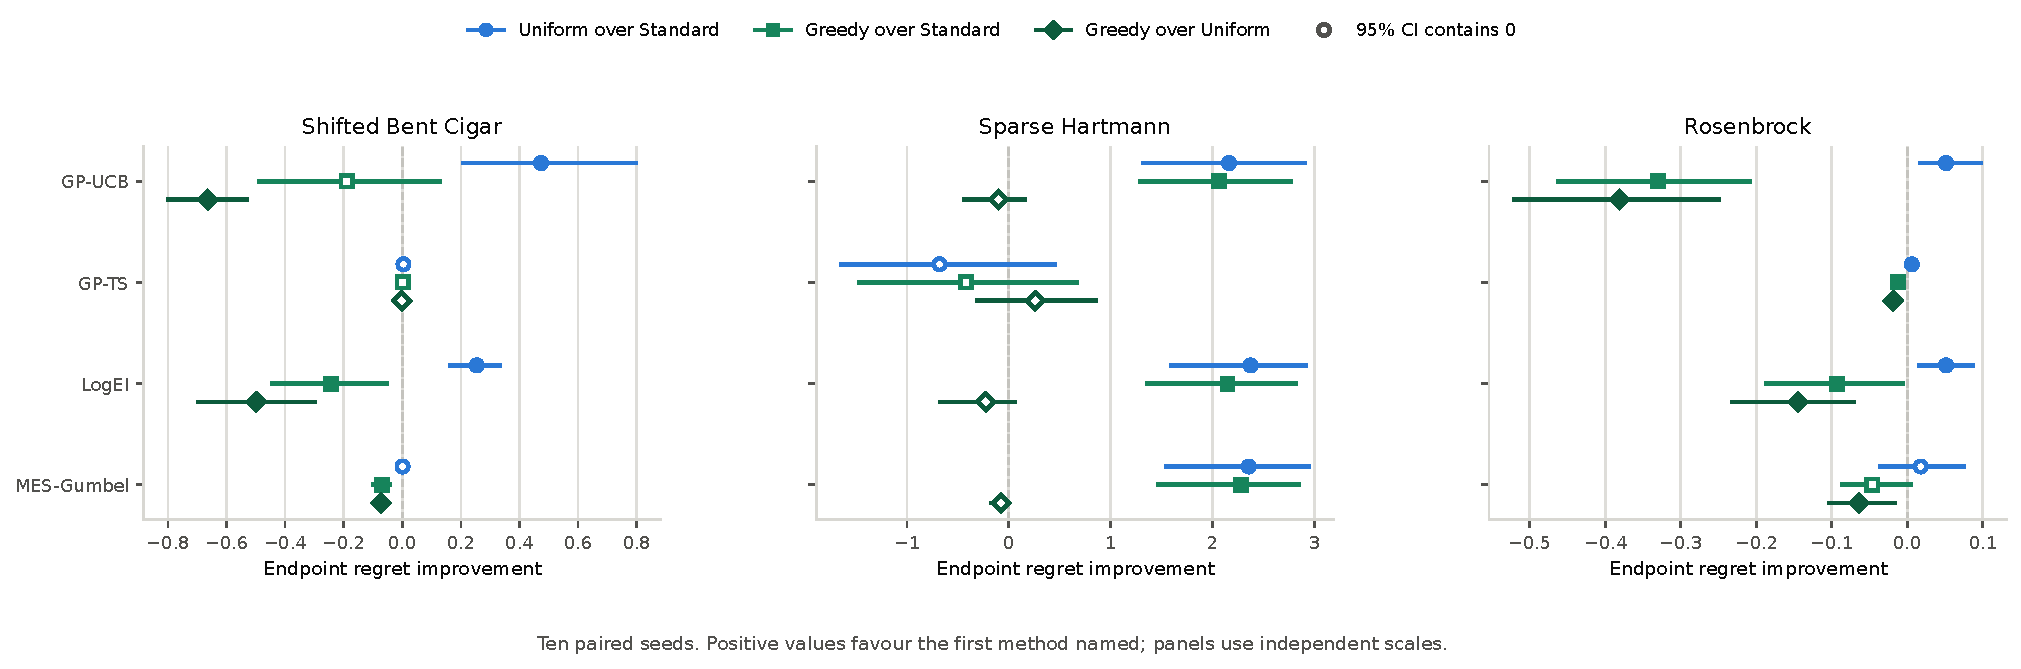
\includegraphics[width=\textwidth]{figures/fig_greedy_packing_acquisition_30d.pdf}
  \caption{Three paired endpoint comparisons in the 30D Greedy Packing study.
  Positive values favor the first method named. Filled markers have paired
  95\% intervals excluding zero; panels use independent horizontal scales.}
  \label{fig:greedypacking30d}
\end{figure}

\begin{table}[H]
\centering
\small
\begin{tabular}{@{}lrrr@{}}
\toprule
Comparison & Better & Inconclusive & Worse \\
\midrule
Uniform over Standard & 8 & 4 & 0 \\
Greedy over Standard & 3 & 4 & 5 \\
Greedy over Uniform & 0 & 5 & 7 \\
\bottomrule
\end{tabular}

\caption{Number of 30D objective--acquisition settings classified by paired
95\% confidence intervals. ``Better'' and ``Worse'' refer to the first method
named in each row.}
\label{tab:greedypacking30d}
\end{table}

\findings\ Uniform PE improves significantly over Standard in 8 of 12 settings
and is never significantly worse. Greedy Packing PE improves in 3 settings,
is worse in 5, and is inconclusive in 4. All three clear Greedy gains occur on
Sparse Hartmann: LogEI, MES-Gumbel, and GP-UCB each improve on all ten paired
seeds. Against Uniform PE directly, Greedy Packing is never significantly
better and is significantly worse in 7 of 12 settings. The broadly positive
Uniform result shows that this is a limitation of the point-selection rule,
not evidence against PE itself.

\subsection{Rastrigin across dimensions}

The second comparison uses rotated shifted Rastrigin in 2D, 5D, 10D, 20D, and
30D with GP-UCB. We reuse 15-seed Standard and Uniform trials and evaluate only
the matching Greedy arm. Each run has 402 total evaluations, including two
initial points. The decay exponents are the values already used in the matched
Uniform study: $1/2$, $1$, $2/3$, $1/2$, and $5/6$, respectively.

\begin{figure}[H]
  \centering
  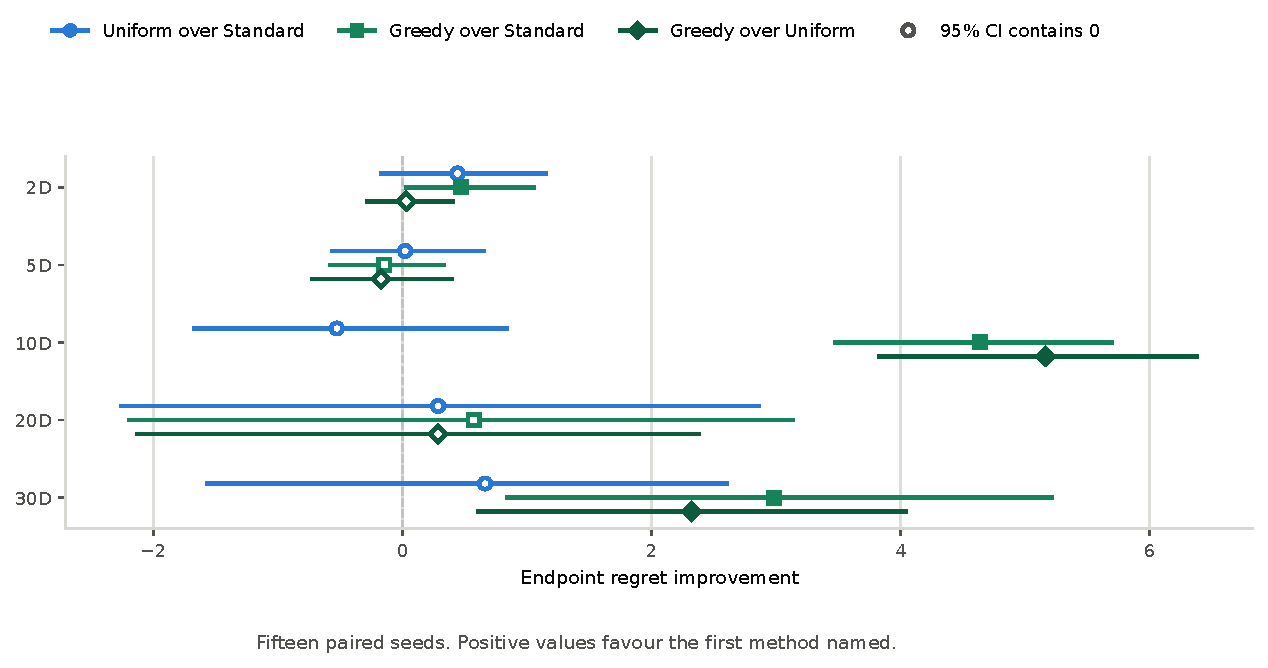
\includegraphics[width=0.75\textwidth]{figures/fig_greedy_packing_rastrigin_dimensions.pdf}
  \caption{Greedy Packing on Rastrigin from 2D to 30D. Positive values favor
  the first method named; filled markers have paired 95\% intervals excluding
  zero.}
  \label{fig:greedypackingdimensions}
\end{figure}

\begin{table}[H]
\centering
\scriptsize
\begin{tabular}{@{}lrrrrrr@{}}
\toprule
Dim. & $\alpha$ & Standard & Uniform & Greedy & G--S & G--U \\
\midrule
2 & $1/2$ & 0.919 & 0.476 & 0.444 & \pewin{+0.475} & \pesoft{+0.032} \\
5 & $1$ & 1.842 & 1.819 & 1.989 & \stdsoft{-0.147} & \stdsoft{-0.170} \\
10 & $2/3$ & 8.022 & 8.548 & 3.381 & \pewin{+4.641} & \pewin{+5.167} \\
20 & $1/2$ & 7.467 & 7.179 & 6.894 & \pesoft{+0.573} & \pesoft{+0.286} \\
30 & $5/6$ & 10.386 & 9.722 & 7.401 & \pewin{+2.985} & \pewin{+2.321} \\
\bottomrule
\end{tabular}

\caption{Mean endpoint inference regret on Rastrigin. G--S and G--U denote
Greedy improvement over Standard and Uniform, respectively. Lower regret and
positive improvement are better.}
\label{tab:greedypackingdimensions}
\end{table}

Greedy Packing clearly improves over Standard in 2D, 10D, and 30D. Its direct
advantage over Uniform is clear in 10D and 30D, with improvements of $5.167$
$[3.813,6.395]$ and $2.321$ $[0.597,4.061]$. The 5D and 20D comparisons are
inconclusive. This confirms that Greedy Packing can be useful, but that its
effect varies with dimension even within one benchmark family.

\subsection{Independent validation of selected settings}

To check that the strongest Rastrigin findings were not caused only by the
original seeds, we fixed one setting for 10D and one for 30D using a separate
five-seed block, then evaluated them on ten new seeds. The fixed settings are
$\alpha=1/2$ with grid-growth coefficient $c=4$ in 10D and $c=16$ in 30D,
where $|G_t|=256+\lceil ct\rceil$. The preliminary setting comparisons are not
included; only the chosen conditions and their fresh-seed evaluation are
reported.

\begin{figure}[H]
  \centering
  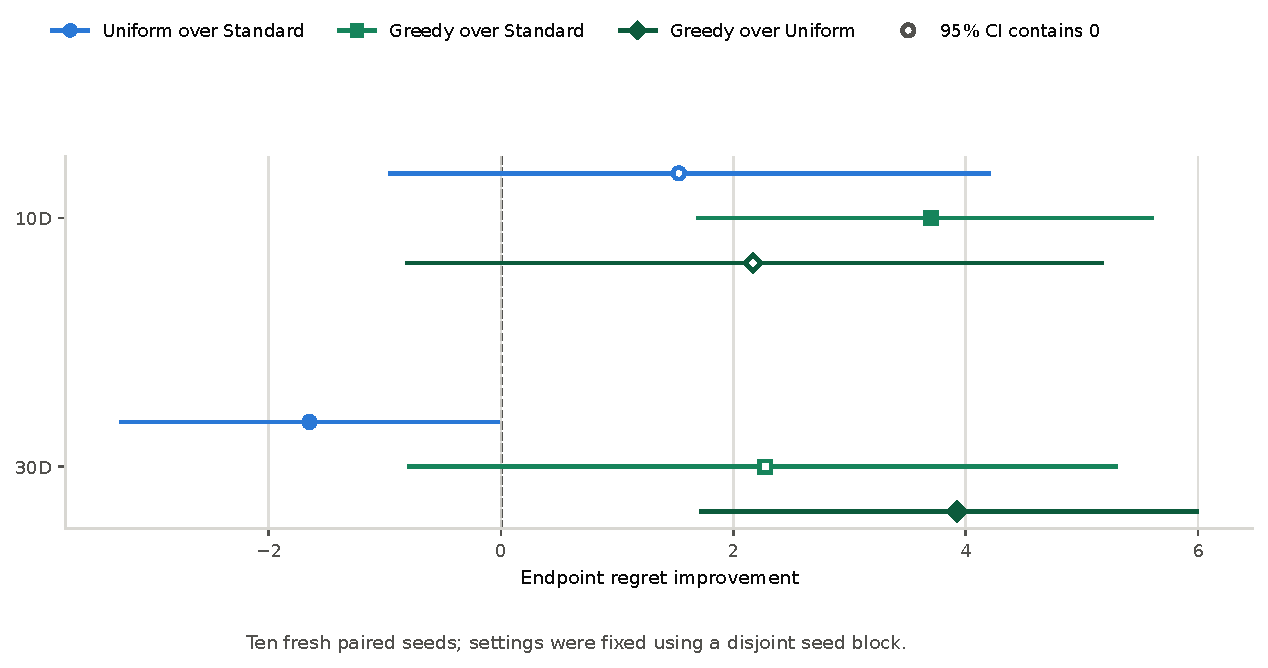
\includegraphics[width=0.75\textwidth]{figures/fig_greedy_packing_rastrigin_validation.pdf}
  \caption{Fresh-seed validation of two fixed Greedy Packing settings on
  Rastrigin. Positive values favor the first method named; filled markers have
  paired 95\% intervals excluding zero.}
  \label{fig:greedypackingvalidation}
\end{figure}

\begin{table}[H]
\centering
\scriptsize
\begin{tabular}{@{}lrrrrrrr@{}}
\toprule
Dim. & $\alpha$ & $c$ & Standard & Uniform & Greedy & G--S & G--U \\
\midrule
10 & $1/2$ & 4 & 8.133 & 6.603 & 4.432 & \pewin{+3.701} & \pesoft{+2.170} \\
30 & $1/2$ & 16 & 7.219 & 8.869 & 4.944 & \pesoft{+2.275} & \pewin{+3.924} \\
\bottomrule
\end{tabular}

\caption{Fresh-seed endpoint results for the selected settings. The grid size
is $256+\lceil ct\rceil$. Lower regret and positive improvement are better.}
\label{tab:greedypackingvalidation}
\end{table}

In 10D, Greedy improves over Standard by $3.701$
$[1.684,5.619]$; its comparison with Uniform is positive but inconclusive. In
30D, Greedy improves over Uniform by $3.924$ $[1.704,6.004]$; its comparison
with Standard is positive but inconclusive. The fresh seeds therefore retain
a Greedy advantage, although the exact significant comparison differs by
dimension.

\subsection{Transfer to Ackley and Rosenbrock}

Finally, we transfer the Rastrigin decay schedule and the default $c=16$
unchanged to Shifted Ackley and Rosenbrock from 2D to 30D. This is an
exploratory five-seed test of whether the Rastrigin result generalizes without
retuning.

\begin{figure}[H]
  \centering
  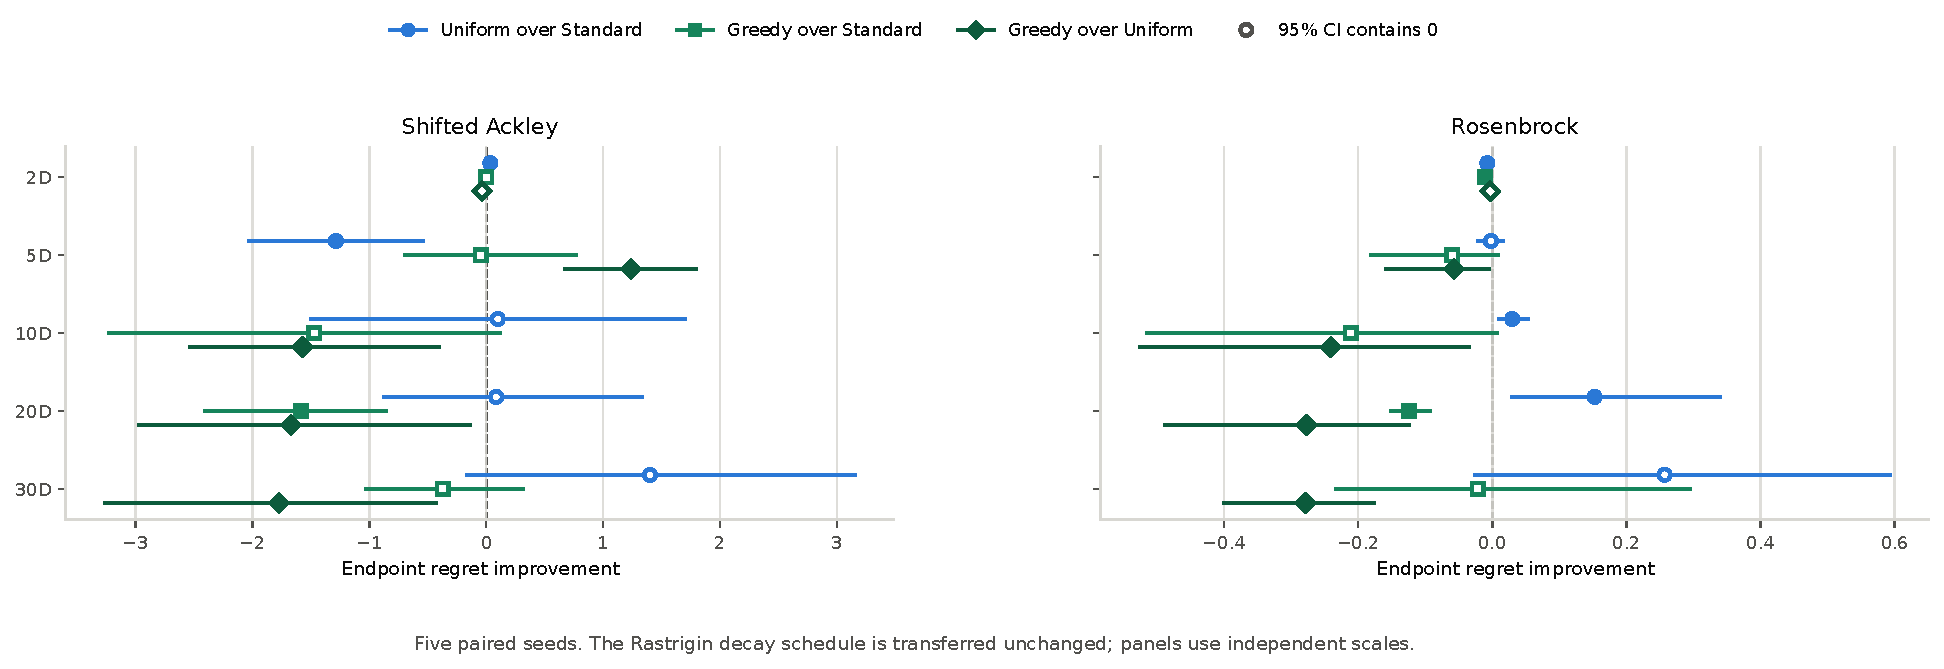
\includegraphics[width=\textwidth]{figures/fig_greedy_packing_cross_benchmark.pdf}
  \caption{Transfer of the Rastrigin Greedy Packing schedule to Shifted Ackley
  and Rosenbrock. Positive values favor the first method named; filled markers
  have paired 95\% intervals excluding zero.}
  \label{fig:greedypackingtransfer}
\end{figure}

\begin{table}[H]
\centering
\small
\begin{tabular}{@{}lrrr@{}}
\toprule
Comparison & Better & Inconclusive & Worse \\
\midrule
Uniform over Standard & 3 & 5 & 2 \\
Greedy over Standard & 0 & 7 & 3 \\
Greedy over Uniform & 1 & 2 & 7 \\
\bottomrule
\end{tabular}

\caption{Number of transferred benchmark--dimension settings classified by
paired 95\% intervals. ``Better'' and ``Worse'' refer to the first method
named in each row.}
\label{tab:greedypackingtransfer}
\end{table}

Greedy is not significantly better than Standard in any of the ten transferred
settings and is worse in three. Against Uniform, it is better once, worse seven
times, and inconclusive twice. Because this stage has only five seeds, it is
best read as a transfer check rather than a final benchmark comparison.

\subsection{Transfer to YAHPO and Lunar Lander}

We next reuse the matched Standard and Uniform arms in the application studies
and evaluate Greedy PE with $\alpha=1/2$. YAHPO uses the same four acquisitions,
tasks, initial designs, budgets, and 30 seeds described in
Section~\ref{sec:hpo}.

\begin{figure}[H]
  \centering
  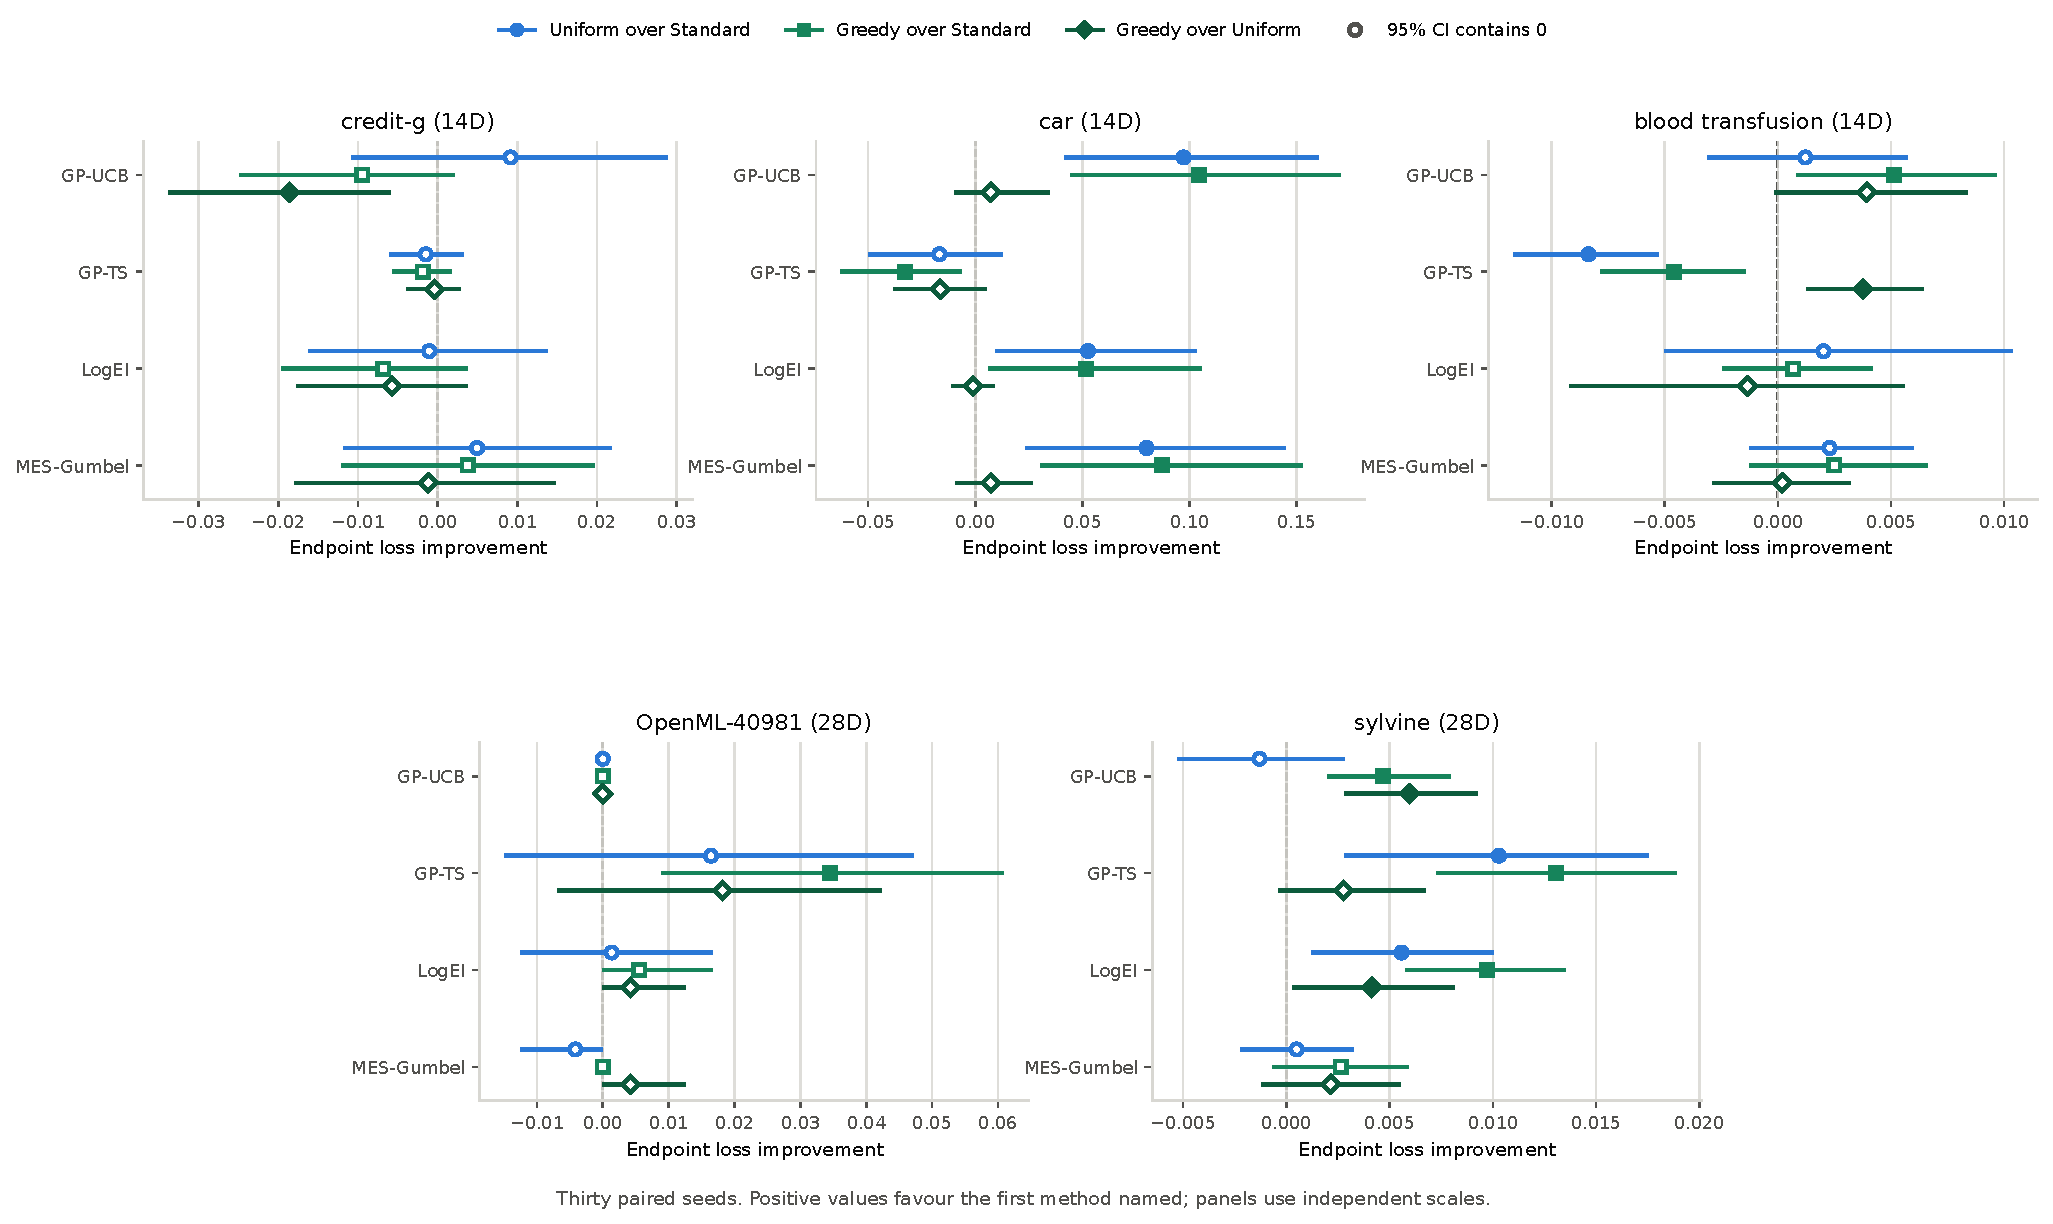
\includegraphics[width=\textwidth]{figures/fig_greedy_packing_yahpo.pdf}
  \caption{Greedy Packing on the 14D and 28D YAHPO tasks. Each panel separates
  the PE effect relative to Standard from the point-rule effect relative to
  Uniform.}
  \label{fig:greedyyahpo}
\end{figure}

In 14D, Greedy improves over Standard in 4 of 12 cells and is worse in 2. In
28D, it improves in 4 of 8 cells with no clear loss. Direct gains over Uniform
occur in only two cells. The 28D result is encouraging, but it does not show a
general Greedy advantage.

The Lunar comparison uses LogEI, 24 initial points, 400 evaluations, and 30
paired seeds. Each BO value averages 50 fixed terrains; the final controllers
are evaluated on 200 shared terrains not used during optimisation.

\begin{figure}[H]
  \centering
  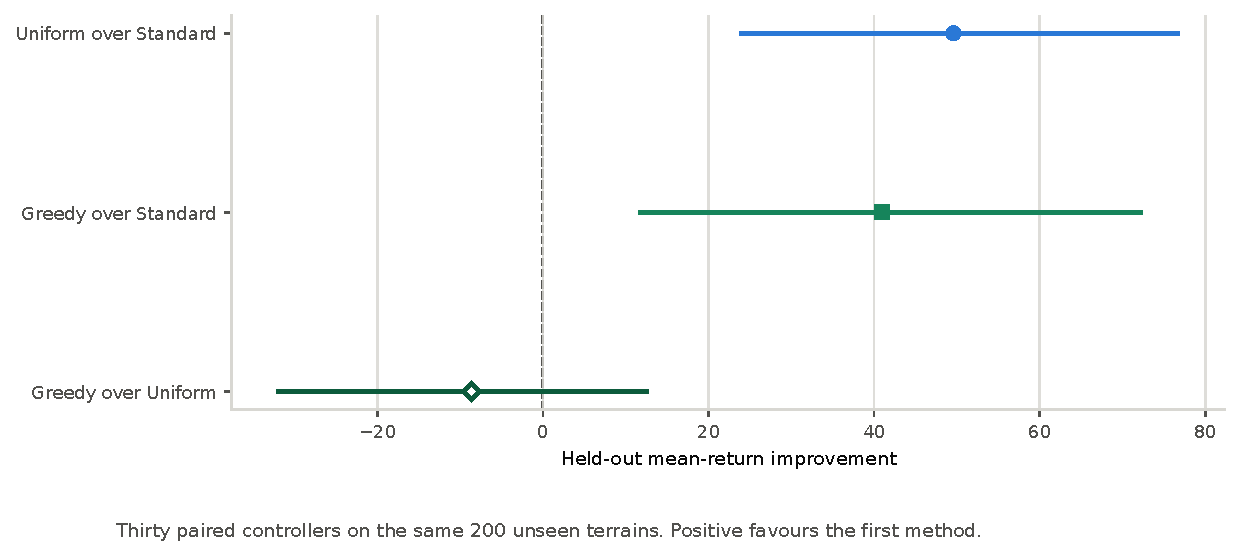
\includegraphics[width=0.72\textwidth]{figures/fig_greedy_packing_lunar.pdf}
  \caption{Paired held-out mean-return comparisons on Lunar Lander.}
  \label{fig:greedylunar}
\end{figure}

Uniform and Greedy improve held-out return over Standard by $+49.6$
$[23.7,76.9]$ and $+40.9$ $[11.6,72.4]$. Solved controllers rise from 20/30
to 27/30 and 24/30. Their direct difference is inconclusive: PE works here,
but Greedy is not better than Uniform.

\subsection{Does a larger finite grid change the conclusion?}

The default grid is a computational choice rather than a fixed property of the
method. We therefore repeat the 30D acquisition panel with the fourfold schedule
$|G_t|=1024+\lceil64t\rceil$, reusing paired Standard and Uniform trajectories.

\begin{figure}[H]
  \centering
  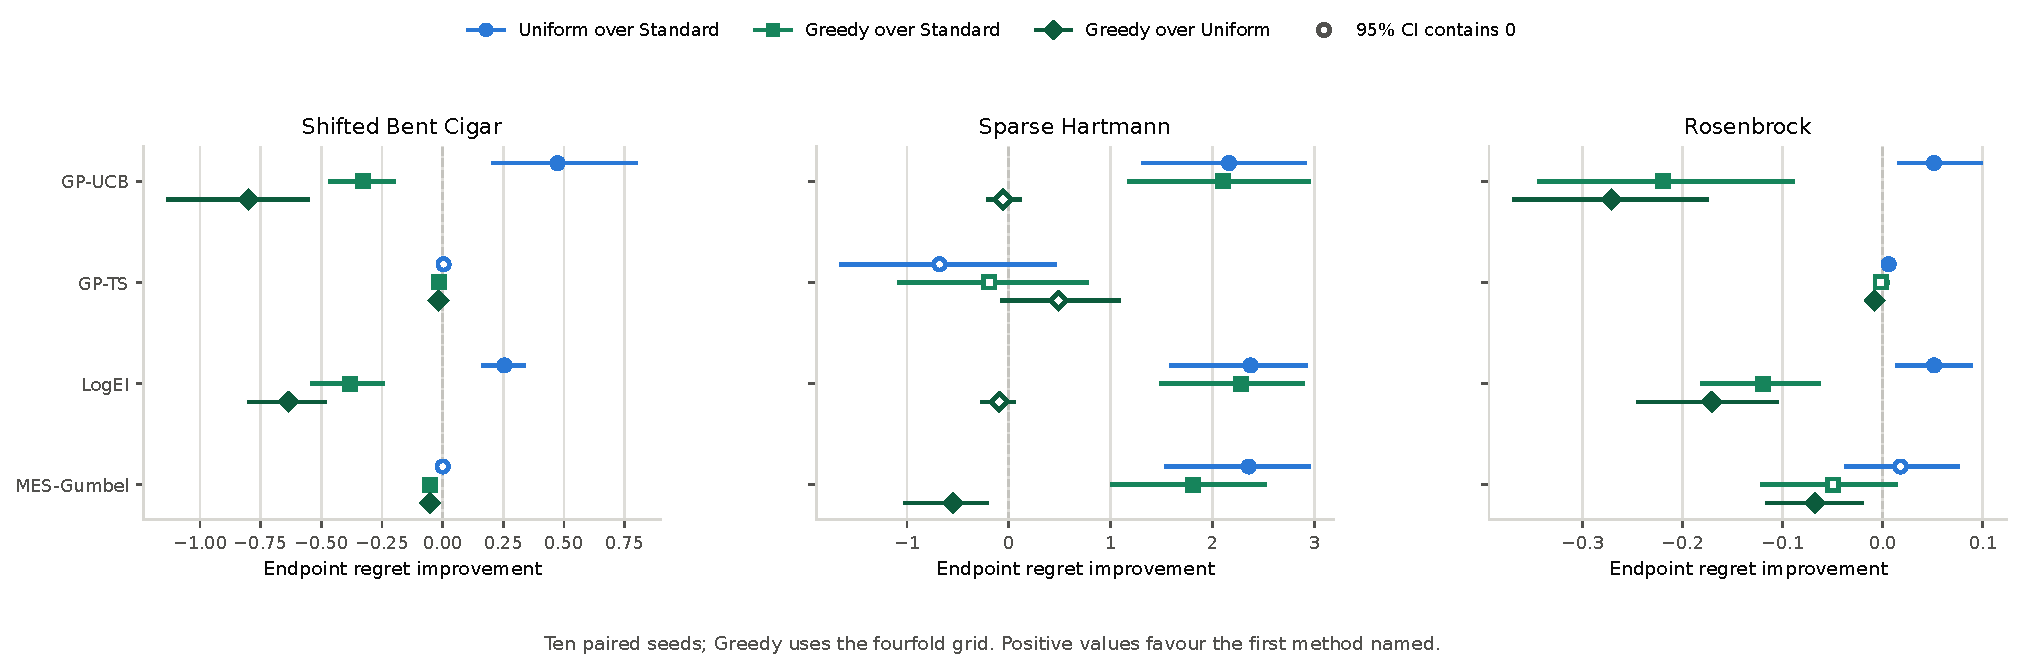
\includegraphics[width=\textwidth]{figures/fig_greedy_packing_acquisition_30d_grid4x.pdf}
  \caption{The 30D acquisition panel with the fourfold Greedy grid. Positive
  values favor the first method named.}
  \label{fig:greedy30dgrid4x}
\end{figure}

Enlarging the grid does not repair the 30D result. Greedy improves over
Standard in 3 cells but is worse in 6; it never clearly beats Uniform and is
worse in 9. Uniform remains the safer rule in this panel.

We then run independent confirmations. The synthetic check uses GP-UCB on
Rastrigin, Ackley, and Rosenbrock in 2D, 10D, and 30D with 15 new seeds. Lunar
uses LogEI and 15 paired seeds. Both compare larger grids with default Greedy
and Uniform under otherwise unchanged BO settings.

\begin{figure}[H]
  \centering
  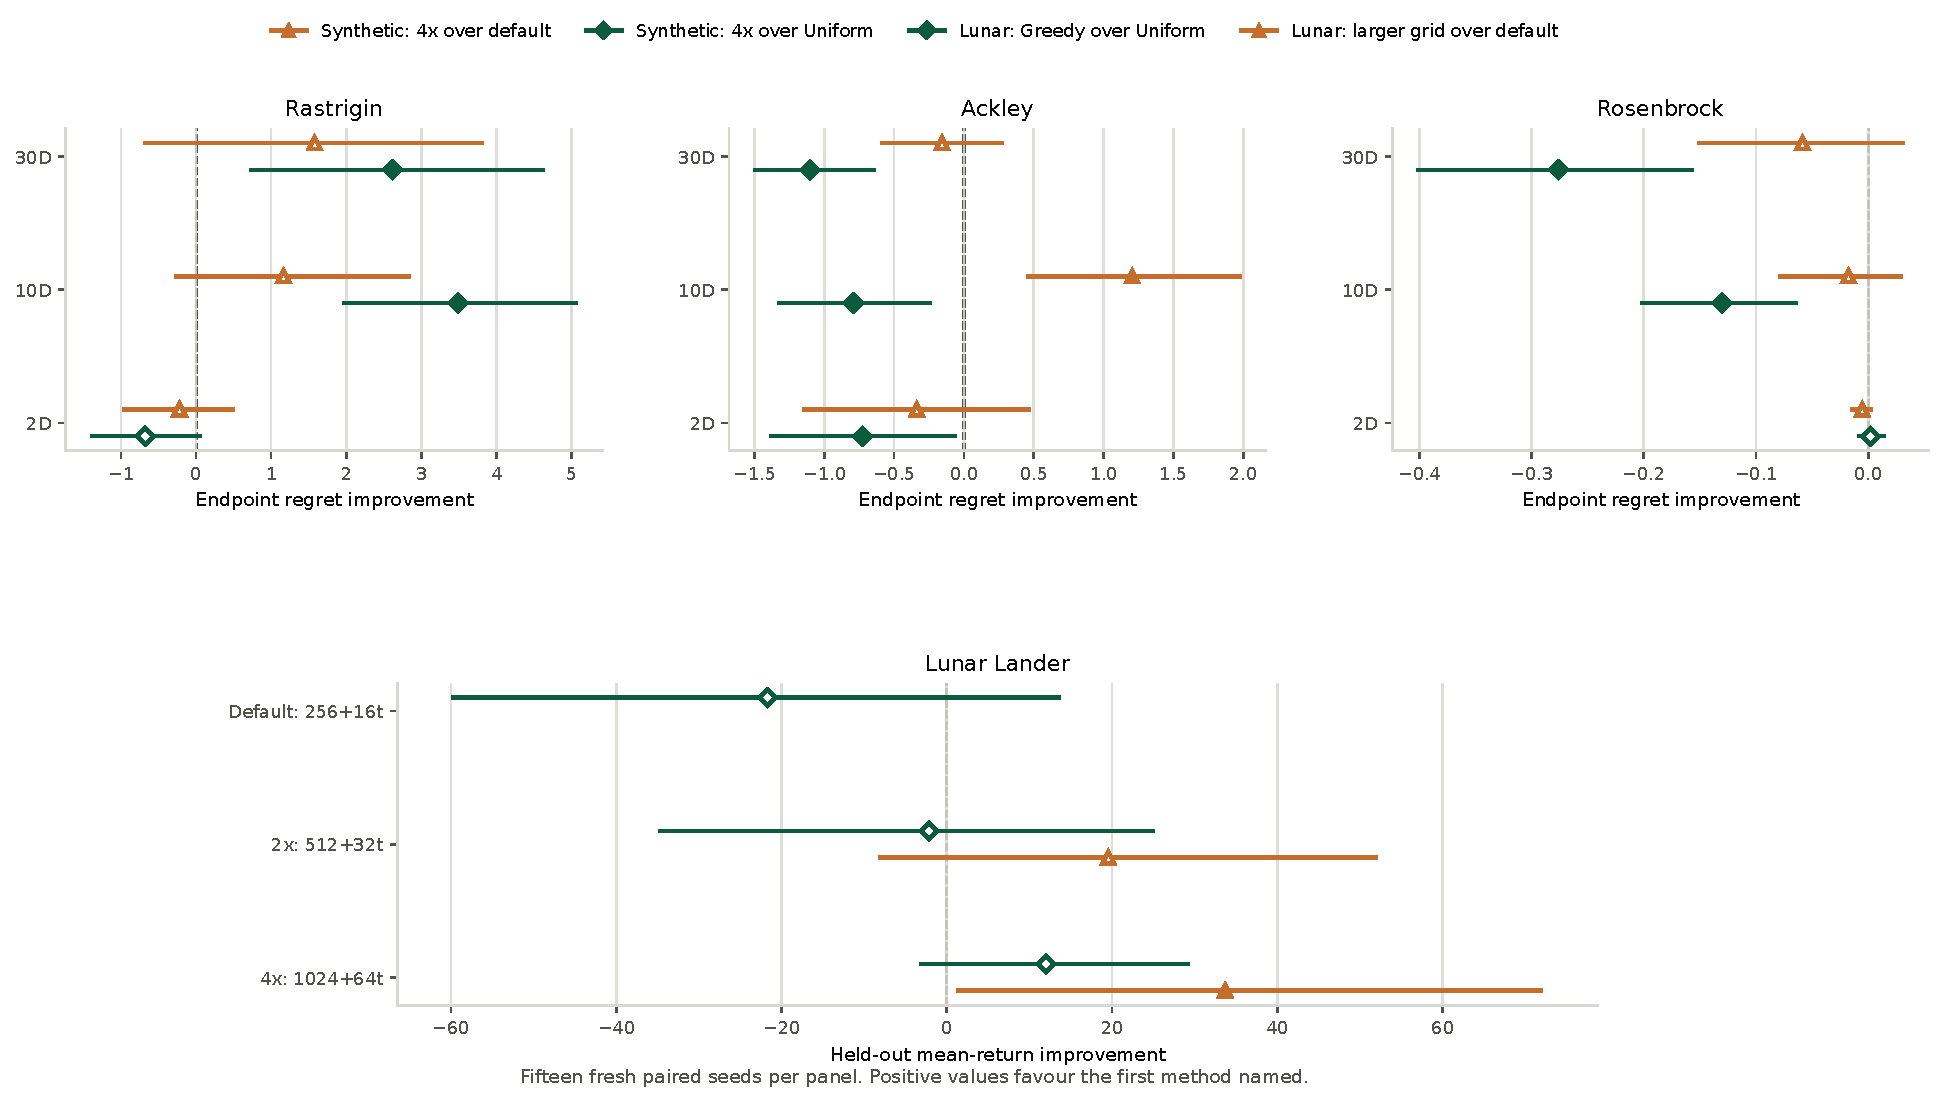
\includegraphics[width=\textwidth]{figures/fig_greedy_grid_confirmation.pdf}
  \caption{Independent large-grid confirmation on synthetic functions and
  Lunar Lander. Filled markers have paired 95\% intervals excluding zero.}
  \label{fig:gridconfirmation}
\end{figure}

The fourfold grid beats Uniform on Rastrigin-10D/30D, but loses on all three
Ackley dimensions and Rosenbrock-10D/30D. On Lunar, it improves over default
Greedy by $+33.7$ $[1.1,72.1]$, but not clearly over Uniform. A larger grid can
repair a coarse approximation on some problems, not make Greedy universally
better.

Finally, Standard, Uniform, and fourfold-grid Greedy are recomputed on 15 fresh
YAHPO seeds with unchanged tasks, acquisitions, initial designs, and budgets.

\begin{figure}[H]
  \centering
  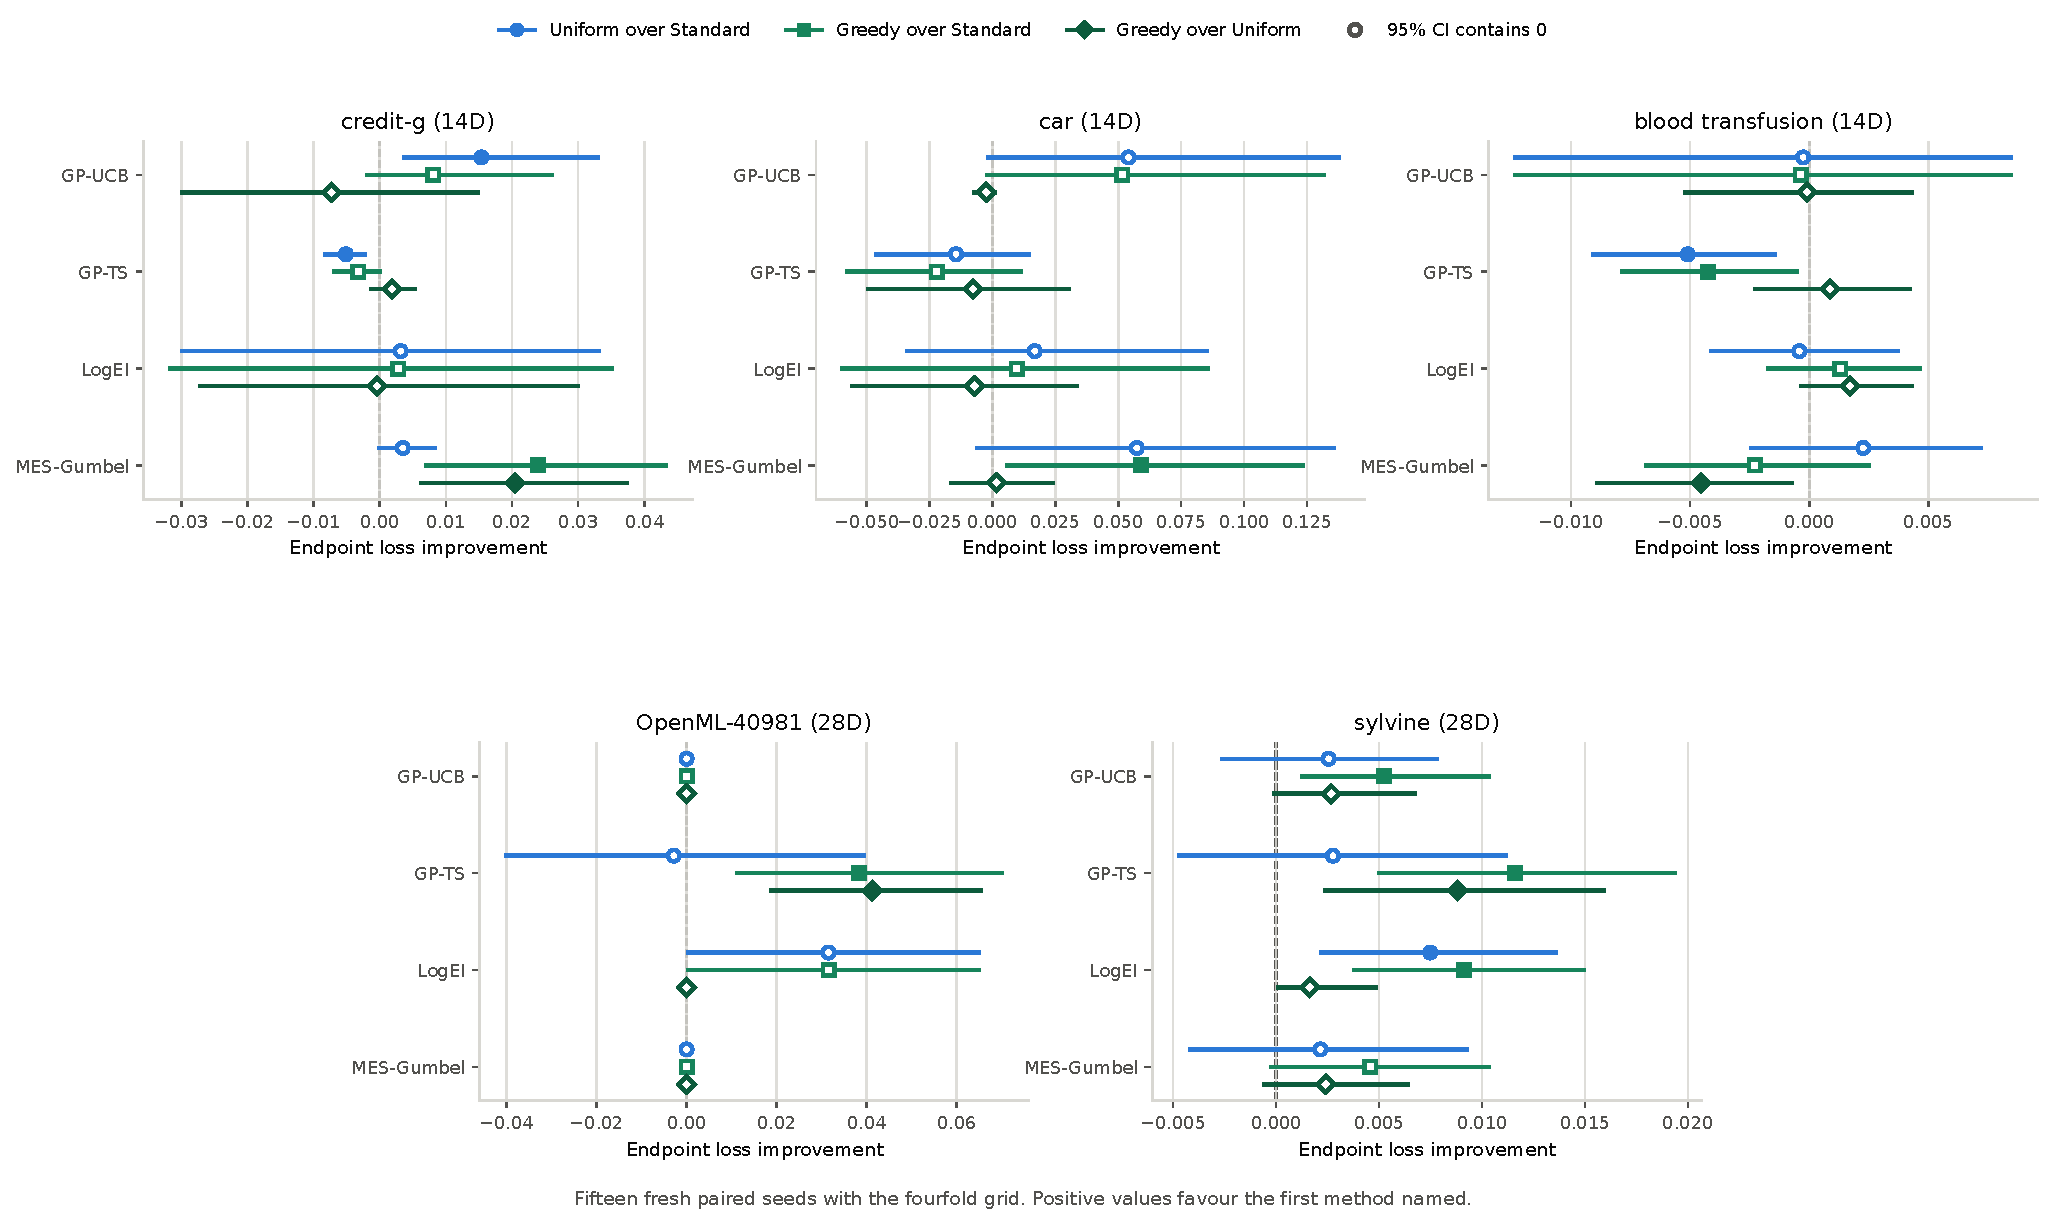
\includegraphics[width=\textwidth]{figures/fig_yahpo_grid4x_confirmation.pdf}
  \caption{Fresh-seed YAHPO confirmation with the fourfold Greedy grid.
  Positive values favor the first method named.}
  \label{fig:yahpogridconfirmation}
\end{figure}

The 14D block remains mixed. In 28D, Greedy improves over Standard in 4 of 8
cells and over Uniform in two GP-TS cells, with no clear loss. The strongest
large-grid evidence is therefore specific to 28D YAHPO.

Overall, Greedy Packing can be effective on Rastrigin and selected 28D HPO
problems, but its gains do not transfer reliably across functions. Increasing
the grid size does not remove this dependence. Uniform sampling therefore
remains the more reliable general-purpose PE rule in the current evidence;
Greedy Packing is a promising problem-dependent option.

\end{document}
